%课题:出淤泥而不染:荷叶的超疏水自清洁性论文:浅析荷叶的超疏水自清洁性

%文档类型
\documentclass[a4paper,12pt]{article}%A4纸,默认字体大小为12pt(小四),文档类型为论文

%宏包
%文字设置
\usepackage[UTF8,heading = true]{ctex}%处理中文
\usepackage{xeCJK}%处理中文
\usepackage{fontspec,xunicode,xltxtra}%字体设置
%文档&排版设置
\usepackage{titlesec}%自定义章节标题样式
\usepackage{multicol}%分栏
\usepackage{hyperref}%超链接设置\daleth 
\usepackage{multirow,makecell}%制作复杂表格
\usepackage{booktabs}%画三线表要用
\usepackage{float}%图片、表格等位置浮动排版
\usepackage{indentfirst}%首行缩进
\usepackage{graphicx,subfigure}%图片插入
\usepackage{listings}%代码高亮
\usepackage{xcolor}
\usepackage{appendix}%附录
\usepackage{fancyhdr}%页眉页脚
\usepackage{geometry}%页边距
\usepackage{caption}
\usepackage{setspace}%局部行距设置
%数学
\usepackage{amsmath,amssymb}%公式
\usepackage{amsfonts,mathrsfs}%数学字体
\usepackage{fontspec}%字体包
\setmainfont{Times New Roman}%让全文英文字体为新罗马字体,同样地,也可以用这种方法改字体为Arial等
%数学字体中起冲突的包为 txfonts, txfonts包的作用是使得全文为 times new roman 字体
%!!!这样英文字体就被锁死,再也无法变动!!!
%解决方法也很简单,调用包时,amsmath一定要在 txfonts包前面
\usepackage{array}%矩阵
\usepackage{gensymb}%角度单位“度”的命令:\degree

\geometry{a4paper,scale=0.8}%设置了纸张为a4,并且版心占页面长度的比例为80%;scale也可以改为ratio,表示版面边距占页面长度的比例. 
\hypersetup{colorlinks=true,linkcolor=black,citecolor=black}%去掉目录等超链接所带的红框,并让参考文献的引用颜色为黑色
\setlength{\parindent}{2em}%首行缩进2字符
\lstset{
    columns=fixed,
    numbers=left, % 在左侧显示行号
    numberstyle=\footnotesize\color{darkgray},% 设定行号格式
    backgroundcolor=\color[RGB]{245,245,244},% 设定背景颜色
    keywordstyle=\color[RGB]{40,40,255},% 设定关键字颜色
    numberstyle=\color[RGB]{0,192,192},%行号数字样式
    commentstyle=\it\color[RGB]{0,96,96},% 设置代码注释的格式
    stringstyle=\rmfamily\slshape\color[RGB]{128,0,0},% 设置字符串格式
}
\pagestyle{fancy}%页眉页脚
\fancyhead{}%清空页眉
\fancyhead[R]{\zihao{-5}{\leftmark}}%页眉右侧为section名(subsection命令为“\rightmark”)
\fancyhead[L]{\zihao{-5}{由荷叶表面的超疏水自洁性展开的思考}}%页眉左侧为标题

%章节名称样式
\CTEXsetup[format={\centering\zihao{3}\heiti}]{section}%设置章标题字号为Large,居中
\CTEXsetup[name={第,章}]{section}%第*章
\CTEXsetup[number={\chinese{section}}]{section}%计数器名称为“section”;chinese格式的序号一,二,三,..

\CTEXsetup[format={\centering\zihao{-3}\heiti}]{subsection}
\CTEXsetup[name={第,节}]{subsection}%第*节                            
\CTEXsetup[number={\chinese{subsection}}]{subsection}%计数器名称为“subsection”

\CTEXsetup[format={\zihao{4}\heiti}]{subsubsection}
\CTEXsetup[name={,、}]{subsubsection}%*、
\CTEXsetup[number={\chinese{subsubsection}}]{subsubsection}%计数器名称为“subsubsection”

%修改目录、参考文献标题样式
\renewcommand\contentsname{\hfill {\zihao{-2}{\heiti 目录}} \hfill}%目录标题居中,用\hfill填充两侧空白

%中英摘要
\newcommand{\enabstractname}{\Large Abstract}%标题
\newcommand{\cnabstractname}{\Large \heiti 摘要}%标题
\newenvironment{enabstract}{%
  \par\small
  \noindent\mbox{}\hfill{\bfseries \enabstractname}\hfill\mbox{}\par
  \vskip 2.5ex}{\par\vskip 2.5ex}
\newenvironment{cnabstract}{%
  \par\small
  \noindent\mbox{}\hfill{\bfseries \cnabstractname}\hfill\mbox{}\par
  \vskip 2.5ex}{\par\vskip 2.5ex}

\newcommand{\suo}{\indent}%缩进2个字符

\title{{\zihao{4}由荷叶表面的超疏水自洁性展开的思考}\footnote{原课题名称为《“出淤泥而不染”:荷叶表面的超疏水自清洁性》}\\\footnotesize{Reflection on the Superhydrophobic Self-cleaning of Lotus Leaf Surface}}%标题
\author{
    \small 江咏宸~~~李佩哲\footnote{按拼音顺序排序,排名不分先后,后同}\\
    \small 指导教师:高鹏\\
    \footnotesize 中国科学技术大学~工程科学学院~近代力学系\\
    \footnotesize 230026\\
    \footnotesize 安徽~合肥}
\date{\small\today}

\setlength{\headheight}{15pt}%为了解决默认字号设为12pt而引发的某些警告
\begin{document}

\maketitle%标题(封面)
\thispagestyle{empty}%不显示页眉页脚

\newpage%分页
\thispagestyle{empty}%不显示页眉页脚
\begin{center}
    \section*{\hfill \heiti{“科学与社会”研讨课课题基本信息} \hfill}%用\hfill填充两侧空白
\end{center}

\begin{table}[H]
    \begin{center}
        \begin{tabular}{|c|c|c|c|}%分四列,每列之间、两边都划竖线(用符号“|”表示);c意为居中
            \hline %划一条一整行的横线
                \multirow{2}*{\textbf{\heiti{小组成员姓名学号}}}&\textbf{\heiti{组员1}}&江咏宸&PB21051050\\%合并两列
                \cline{2-4}&\textbf{\heiti{组员2}}&李佩哲&PB21051049\\%在第2-4列划横线
            \hline
                \textbf{\heiti{课题名称}}&\multicolumn{3}{c|}{由荷叶表面的超疏水自洁性展开的思考}\\
            \hline
                \multicolumn{4}{|c|}{\textbf{\heiti{研究背景及意义}}}\\
            \hline
                \multicolumn{4}{|c|}{\makecell{\\\parbox{16.8cm}
                {~~~~~~~20世纪90年代,德国的两位科学家率先用扫描电镜观察了荷叶的表面结构,认为“自清 洁”效应是由荷叶表面上的微米级乳突及表面蜡状物共同引起的. 之后又有人进行了进 一步的研究,发现荷叶表面乳突上还存在纳米结构,这种微米与纳米结构同时存在的二 元结构才是引起荷叶表面“自清洁”的根本原因. 本研究试图站在巨人的肩膀上,重走 先辈之路,并尝试是否能有其他的发现. }\\~}}\\
            \hline
                \multicolumn{4}{|c|}{\textbf{\heiti{研究内容}}}\\
            \hline
                \multicolumn{4}{|c|}{\makecell[l]{了解荷叶表面微观结构,并从实验上证明其疏水性,理实交融;\\
                    观察在水滴的撞击荷叶表层时的发生变化;\\
                    探究其它类型的疏水材料的性质;\\
                    尝试对液滴在某种表面上的形状做出模拟与预测. }}\\
            \hline
                \multicolumn{4}{|c|}{\textbf{\heiti{项目分工}}}\\
            \hline
                \multicolumn{4}{|c|}{
                    \begin{tabular}{l|c}
                        \makecell[l]{江咏宸:\\
                        1.查找资料 \\
                        2.进行实验 \\
                        3.共同撰写论文、PowerPoint}
                        &\makecell[l]{李佩哲:\\
                        1.电子文稿排版 \\
                        2.进行实验 \\
                        3.共同撰写论文、PowerPoint}
                    \end{tabular}
                }\\
            \hline
                \multicolumn{4}{|c|}{\textbf{\heiti{研究计划}}}\\
            \hline
                \multicolumn{4}{|c|}{\makecell[l]{联系相关实验室,取得基础实验条件;\\
                实验探究,证明荷叶的疏水性,探究其它疏水材料的性质;\\
                进行液滴形状分析,了解原理与过程;\\
                撰写论文,宏观调控;\\
                总结经验,做好结项工作. }}\\
            \hline
                \multicolumn{4}{|c|}{\textbf{\heiti{预期研究成果}}}\\
            \hline
                \multicolumn{4}{|c|}{\makecell[l]{深入了解荷叶超疏水自清洁原理,对其纳米结构有一定的了解;\\
                学习掌握Young-Laplace方程及其推论,学会进行液滴形状分析;\\
                熟练掌握使用Matlab、$\LaTeX$等辅助工具的用法. }}\\
            \hline
        \end{tabular}
    \end{center}
\end{table}

\newpage%分页
\thispagestyle{empty}%不显示页码
\begin{spacing}{1.528}%段落行距设置
\begin{cnabstract}%中文摘要
    人们对荷叶的超疏水性的研究由来已久. 本文立足于前人研究的基础上,对荷叶超疏水性的成因、状态、应用进行了研究. 
    本课题调查了已经公布的研究成果,并进行了实验探究,在验证已有结论的同时,将对液滴形状的预测机械化,成功模拟并预测了液滴在表面的状态. 
    另外,本课题也进行了扩展,对水滴下落击中荷叶前后状态的变化、荷叶表面的疏油性能等方面进行了广泛的实验探究,取得了较好的结果. 
\\\textbf{关键词:}荷叶、超疏水性、自清洁性、Young-Laplace方程、ADSA
\end{cnabstract}

\begin{enabstract}%英文摘要
    The superhydrophobic properties of lotus leaves have been studied for a long time. 
    Based on previous studies, this paper studied the cause, state and application of lotus leaf superhydrophobic. 
    The subject investigated the published research results and conducted experimental exploration. 
    While verifying the existing conclusions, the prediction of droplet shape was mechanized, and the state of droplet on the surface was successfully simulated and predicted. 
    In addition, this subject has also been expanded, and extensive experimental research has been carried out on the changes of the state before and after the water drops hit the lotus leaf, the oil drainage performance of the lotus leaf surface, and good results have been achieved.
\\\textbf{Keywords:}lotus leaf, superhydrophobic, self-cleaning, Young-Laplace equation, ADSA
\end{enabstract}
\end{spacing}

\newpage%分页
\setcounter{page}{1}%从这开始标页码
\thispagestyle{empty}%不显示页眉页脚
\tableofcontents%生成目录
\thispagestyle{empty}%不显示页眉页脚
\newpage

%\begin{multicols}{2}%分栏

\section{绪论}%一级标题
\subsection{研究背景}%二级标题
\begin{spacing}{1.528}%段落行距设置
自然状态下,水滴滴落在荷叶表面时并不会浸润荷叶自身,而是会以水珠的形式存在,并且极易滑落,这便是荷叶的超疏水性. 
同样的现象也可以在水黾等处看到. 另外,水珠的滚动可以吸附荷叶表面的杂质,实现荷叶表面的自清洁. 
自古以来,人们就对这种现象心怀好奇,并尝试制备具有类似性质的材料. 
鉴于此,对荷叶表面超疏水自清洁性质的探究与了解对新时代大学生拓展眼界、学习知识、提升水平大有裨益. 

周敦颐在《爱莲说》中曾说:「莲之出淤泥而不染」,这正是大自然中神奇的地方. 通过查阅文献和资料
可以知道,由于莲叶具有疏水、不吸水的表面,落在叶面上的雨水会因表面张力的作用形成水珠,
换言之,水与叶面的接触角会大于150\degree(接触角大于150\degree),只要叶面稍微倾斜,水珠就会滚离叶面(滚动角小于20\degree)
$^\text{\cite{ref1,ref2,ref3,ref4,ref5,ref6,ref7}}$. %在正文中引用参考文献
因此,即使经过一场倾盆大雨,莲叶的表面总是能保持干燥;此外,滚动的水珠会顺便把一些灰尘污泥的颗粒一起带走,达到自我洁净的效果,这就是莲花总是能一尘不染的原因. 

巴特洛特等人在显微镜下发现,莲叶的表面有一层茸毛和一些微小的蜡质颗粒,水在这些纳米级的微小颗粒上不会向莲叶表面其他方向蔓延,而是形成一个个球体,就是莲叶上滚动的雨水或者露珠,这些滚动的水珠会带走叶子表面的灰尘,从而清洁了叶子表面. 
\end{spacing}

\subsection{研究目的和意义}
\begin{spacing}{1.528}%段落行距设置
本研究旨在站在巨人的肩膀上,重走先辈之路,拓宽眼界、增长见识、获得新知,并在尝试获得新的发现的同时,学习进行科学研究的一般方法、步骤和理论,为将来参与科研工作奠定坚实基础. 
\end{spacing}
\subsection{研究方法}
\begin{spacing}{1.528}%段落行距设置
鉴于本研究的目的和意义,以及研究背景,课题小组决定通过以查阅文献与理论计算为主,以简要实验为辅,再加上Matlab计算与作图,几种方法齐头并进,从不同角度进行探究与学习. 
\end{spacing}

\section{理论基础}

\subsection{表面张力}
\begin{spacing}{1.528}%段落行距设置
水等液体会产生使表面尽可能缩小的力,这个力称为“表面张力”
$^\text{\cite{ref7.5}}$. 

由于表面张力仅在液体自由表面或两种不能混合的液体之间的界面处存在,一般用表面张力系数$\gamma$来衡量其大小. $\gamma$表示表面上单位长度所受拉力的数值,单位为$N/m$. 液体的表面张力系数,是液体本身的一种性质,主要由液体本身决定. 
在没有特别说明的情况下,本文所说的“表面张力”均指表面张力系数$\gamma$. 
\end{spacing}

\subsection{接触角}
\subsubsection{杨氏接触角与杨氏方程}
\begin{spacing}{1.528}%段落行距设置
接触角是指在固、液、气三相交界处,自固-液界面经过液体内部到气-液界面之间的夹角
$^\text{\cite{ref8}}$. 
根据力的平衡,液滴在平面上的接触角由气固($\gamma_{gs}$),气液($\gamma_{lg}$),液固($\gamma_{ls}$)三者表面张力决定. 
即杨氏方程
\begin{equation}
    \gamma_{gs}=\gamma_{ls}+\gamma_{lg}\cos\theta_{Y}
\end{equation}
其中$\theta_Y$为杨氏接触角. 
\end{spacing}

\subsection{Cassie状态和Wenzel状态}
\subsubsection{Cassie状态}
Cassie状态(图\ref{Cassie})%在正文中引用图片
表明液体与固体间不完全接触,存在气体(一般称为“气垫”或“气室”(gas chamber))

\begin{figure}[H]%插入图片
    \centering%图片居中
    \subfigure[Cassie状态]{%小图一的名称
        \includegraphics[scale=0.5]%图片大小(原始图片的百分之几)
        %几个参数:
            %height 图形的高度(可为任何 TEX 度量单位). 
            %totalheight    图形的全部高度,可为任何 TEX 度量单位( 6/95 增加). 
            %width  图形的宽度(可为任何 TEX 度量单位). 
            %scale	图形的缩放因子,设定 scale=2 会使 插入的图形的大小为其自然大小的两倍. 
            %angle	设定旋转的角度,以度为单位,顺时钟方向为正. 
            %origin	指定图形绕那一点旋转,缺省是图形的参考点(12/95 增加). 初始点有可能与\rotatebox命令中的一样.  比如 origin=c 将使图形绕它的中心旋转. 
        {图像/Cassie.png}%相对路径(不在同一文件夹下用绝对路径)
        %注意!!!!!:一般在论文中应插入格式为.eps的矢量图!!!!!
        \label{Cassie}%用于引用的标签
        }
    \quad
    \subfigure[Wenzel状态]{%小图二的名称
        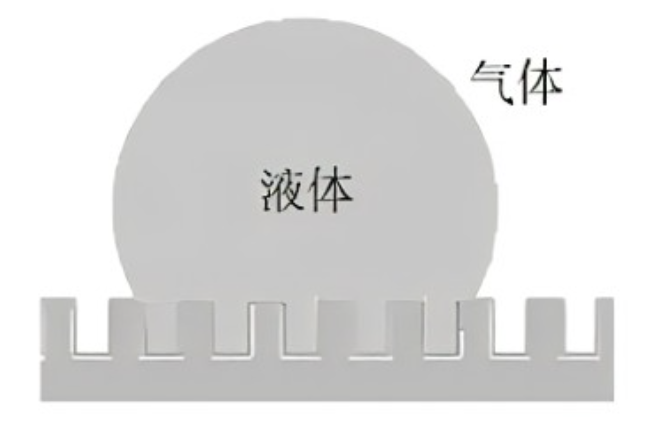
\includegraphics[scale=0.5]{图像/Wenzel.png} \label{Wenzel} 
        }
    \caption{液体在粗糙有空固体表面的两种状态}%总的图名称
\end{figure}

\subsubsection{Wenzel状态}
Wenzel状态(图\ref{Wenzel})下液体与固体紧密接触,界面不包含气体. 

\subsubsection{Cassie模型与Wenzel模型的理论与发展}
\begin{spacing}{1.528}%段落行距设置
实 验 观 察 发 现 自 然 界 的 超 疏 水 现 象 是 由 纳 微 结 合 的 粗糙 表 面 引 起 的 , 液 滴 在粗糙 表 面 的 接 触 角 不 能 用 杨 氏 方 程 来 描 述 . 
Wenzel等人首先对粗糙表面的液滴进行了研究,发现液滴在具有粗糙度的固体表面形成均匀的润湿状态(如图\ref{Wenzel}),
粗糙度的存在使得亲水固体表面表现出更强的亲水作用,疏水固体表面表现出更强的疏水作用,其理论方程可表示为
\begin{equation}
    \cos\theta_W=r\cos\theta_Y
\end{equation}
其中$\theta_W$为Wenzel态的表观接触角,$r$为粗糙度. (利用液滴能量最小可得此方程
$^\text{\cite{ref9}}$. )
另一方面,Cassie等人则发现了另外的液滴润湿状态(如图\ref{Cassie}),液滴在固体表面形成固-气、固-液的复合接触表面,使得液滴的接触角大大增加,
其理论方程可表示为
\begin{equation}
    \cos\theta_C=f_s\cos\theta_{Y,1}+f_v\cos\theta_{Y,2}
\end{equation}
其中$\theta _C$为Cassie态表观接触角,$f_s,f_v$分别为固相和气相所占体积分数,如$f_s$为固-液总面积除以总投影面积. 
因此对于均匀分布且规则的粗糙度,存在$f_s+f_v=1$;但对于具有不规则形状的固体基质——例如三角形——则并不一定满足$f_s+f_v=1$. 
(Cassie模型同样可由液滴的最小能量得到
$^\text{\cite{ref9}}$. )
\end{spacing}

\subsection{滚动角}
\begin{spacing}{1.528}%段落行距设置
滚动角,又称滑移角,与接触角相类似,是表征一个特定表面润湿性的重要方法. 也是常用的一种测量材料表面润湿性的方法
$^\text{\cite{ref17}}$. 
滚动角是指液滴在倾斜表面上刚好发生滚动时,倾斜表面与水平面所形成的临界角度.
液 滴 在 疏 水 表 面 具 有 大 的 接 触 角 ,虽 然 可以 有 效 地 减 小 固 液 之 间 的 接 触 面 积,
但有的情况下,即使液滴有大于150$^{\circ}$的接触角,但液滴仍然难以移动,如玫瑰花效应:
玫瑰花瓣表面静态水滴接触角与荷叶表面类似,但是具有较高的接触角滞后,使得水滴在其表面呈现超粘附状态,从而实现花瓣的长久保鲜
$^\text{\cite{ref18}}$. 
因此液滴在超疏水表面的滑动难易程度主要是由粗糙度提供的锚定决定. 
\end{spacing}

\subsection{Young-Laplace方程}
\begin{spacing}{1.528}%段落行距设置
杨-拉普拉斯方程式是一个非线性偏微分方程,可以用来计算两静态流体界间因表面张力或壁张力造成的毛细管压力差,如水与空气之间的
$^\text{\cite{ref21}}$. 

杨-拉普拉斯公式是指物理中的附加压力$p_s$与曲率半径$R$之间的关系式
\begin{equation}
    p_s=\gamma\left(\frac{1}{R_1}+\frac{1}{R_2}\right)\label{young}
\end{equation}
其中$\frac{1}{R_1},\frac{1}{R_2}$为液面的主曲率. \\特殊情况下,即$R_1=R_2=R$时,有
\begin{equation}
    p_s=\frac{2\gamma}{R}\label{ps}
\end{equation}
\end{spacing}

\subsection{ADSA}\label{adsa}
\begin{spacing}{1.528}%段落行距设置
ADSA,全称Axisymmetric Drop Shape Analysis,即轴对称液体形状分析,一般是通过Young-Laplace方程及其推论,在弧长坐标系下求解一个常微分方程组的数值解,
从而获得液滴理论形状
$^\text{\cite{ref22}}$. 

首先,给出Young-Laplace方程式
\begin{equation}
    \Delta p=\gamma\left(\frac{1}{R_1}+\frac{1}{R_2}\right)\label{laplace}
\end{equation}
这里用相对于水平面的压力的变化量$\Delta p$代替了式\eqref{young}中附加压力$p_s$,含义不变. 
在没有重力以外的外力的情况下,$\Delta p$是相对高度的线性函数
\begin{equation}
    \Delta p=\Delta p_0+(\Delta \rho )gz
\end{equation}
其中$\Delta p_0$是参考平面上的压力差(附加压力),$\Delta\rho$是两个主体相(气相与液相)之间的密度之差,$g$是重力加速度,$z$指液滴上指定点到参考平面的垂直高度差(海拔差). 
因此,对于给定的$\gamma$,可以针对已知的物理属性值(即密度和重力)和已知几何量(即主曲率$R_1$和$R_2$)来确定液滴的形状. 反之 ,根据液滴形状确定界面张力$\gamma$,或是用全部已知数据取拟合水滴形状从而精确测量接触角,原则上也是可能的;然而,这是一项更加艰巨的任务
$^\text{\cite{ref22,ref23}}$. 

以确定液滴的形状为例,式\eqref{laplace}描述了被界面分隔的两种均匀流体的机械平衡条件. 对于一个轴对称的固-液界面(如图\ref{ADSA}),主曲率半径$R_1$与界面的弧长和水平方向的倾角$\phi$之间的关系为
\begin{equation}
    \frac{1}{R_1}=\frac{\text d\phi}{\text ds}\label{r1}
\end{equation}
其中$\phi$为界面相对于水平方向($x$轴方向)的夹角,$s$为沿界面的弧长. 
\begin{figure}[H]
    \centering
    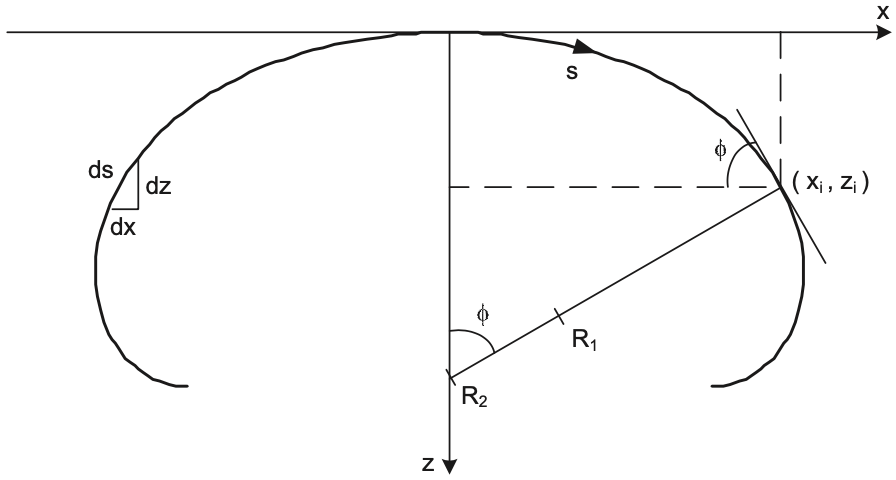
\includegraphics[scale=0.38]{图像/ADSA.png}
    \caption{ADSA的标准坐标系建系方法}\label{ADSA}
\end{figure}
第二个主曲率半径$R_2$则由以下公式给出:
\begin{equation}
    \frac{1}{R_2}=\frac{\sin\phi}{x}\label{r2}
\end{equation}
\suo 由于研究对象的界面是轴对称的,所以顶点处的曲率在所有方向上都是恒定的,并且两个主曲率(主曲率半径)相等,即$s=0$时,有
\begin{equation}
    \frac{1}{R_1}=\frac{1}{R_2}=\frac{1}{R_0}=b
\end{equation}
其中$R_0$和$b$分别为原点(如图\ref{ADSA}中$x=0,z=0$)处的曲率半径和曲率. 因此根据式\eqref{laplace},原点处的压差可以表示为
\begin{equation}
    \Delta p_0=2b\gamma\label{p0}
\end{equation}
这与式\eqref{ps}相同. 

将式\eqref{r1}\eqref{r2}\eqref{p0}代入式\eqref{laplace},并定义毛细管常数(capillary constant)$c$\footnote{另外一个概念:毛细管数(Capillary number,Ca),亦称界面张力数,是一个无量纲量,最初由Taylor于1934年提出. 毛细管数定义为流体粘性力和界面张力的比值. 在流体力学中,常用毛细管数和两相粘度比来表征预测两相流体中分散相液滴的形变和破裂发生的程度和可能性
$^\text{\cite{ref24}}$. }
,得
\begin{equation}
    \frac{\text d\phi}{\text ds}=2b+cz-\frac{\sin\phi}{x}\label{ph}
\end{equation}
\begin{equation}
    c=\frac{(\Delta\rho)g}{\gamma}\label{c}
\end{equation}
对于固着液滴,毛细管常数$c$为正值,而对于悬垂液滴,毛细管 常数$c$为负值. 式\eqref{c}与几何关系
\begin{equation}
    \frac{\text dx}{\text ds}=\cos\phi\label{x}
\end{equation}
\begin{equation}
    \frac{\text dz}{\text ds}=\sin\phi\label{z}
\end{equation}
一起,建立了一组关于$x$,$y$和$\phi$的一阶微分方程,以此作为弧长$s$的函数. 

在边界条件
\begin{equation}
    x(0)=z(0)=\phi(0)=0
\end{equation}
下,同时有$s=0$,此时
\begin{equation}
    \frac{\text d\phi}{\text ds}=b\label{b}
\end{equation}

对于给定确定数值的$b$和$c$,通过求解上述\eqref{ph}\eqref{c}\eqref{x}\eqref{z}\eqref{b}等构成的常微分方程组,可以得到拉普拉斯轴对称流体-液体界面的完整形状. 
\end{spacing}

\section{研究假设}
%第三章是在第二章的理论基础上,论述你提出了怎样的研究假设. 也是你整篇文论的核心观点. 
\begin{spacing}{1.528}%段落行距设置
根据$\mathfrak{Section}~\uppercase\expandafter{\romannumeral2}$的理论基础,结合研究目的与对象,提出了以下几点假设:
\begin{enumerate}
    \item 荷叶表面有纳微级的凸起/孔洞结构,使得空气进入其中形成气垫,荷叶表面疏水层与水滴之间的状态类似于Cassie状态(如图\ref{Cassie});
    \item 荷叶表面还具有自清洁性等其他性质;
    \item 可以根据水珠在一般表面的状态来计算接触角,也可以通过接触角来推断水珠在一般表面的形状. 
\end{enumerate}
\end{spacing}

\section{研究过程}
%一般是在第三章提出研究假设的基础上,对收集来的数据进行分析的过程,以验证你的假设是否成立. 
\subsection{对于荷叶表面性质的探究}
\subsubsection{样本采集}
\begin{spacing}{1.528}%段落行距设置
从中国科学技术大学东校区眼镜湖采集荷叶,清洗干净,获取实验样品. 
在此为课题组未经允许采集荷叶的行为致歉. 
在清理过程中,就已经发现水珠在荷叶上表面滚动而未留丝毫痕迹. 
\end{spacing}

\subsubsection{水滴在荷叶表面的状态}
\begin{spacing}{1.528}%段落行距设置
对样本进行简要处理后,切块,分别进行不同的实验. 
接触角的测量结果如图\ref{水滴接触角图}所示,可以观察到,体积较小的水珠在荷叶表面近似呈球状,接触角为145\degree,证明了荷叶表面的超疏水性;
而体积较大的水珠在荷叶表面由于重力作用而被“压扁”,但接触角也近似在145\degree. 
\end{spacing}

\begin{figure}[H]
    \centering
    \subfigure[小水滴在荷叶表面状态]{
        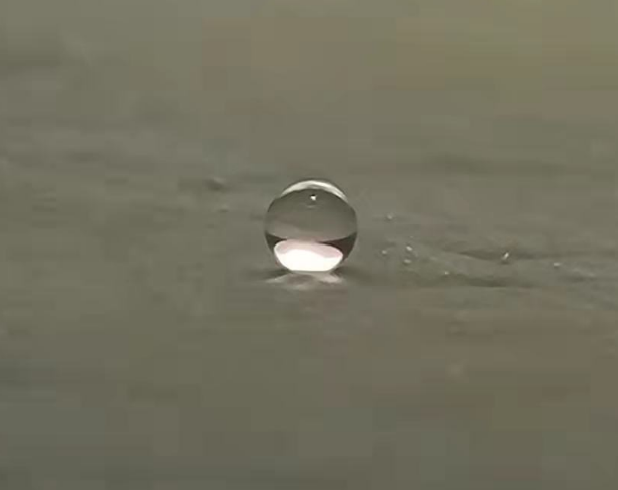
\includegraphics[scale=0.125]{图像/小水滴.png}
        }
    \quad
    \subfigure[大水滴在荷叶表面状态]{
        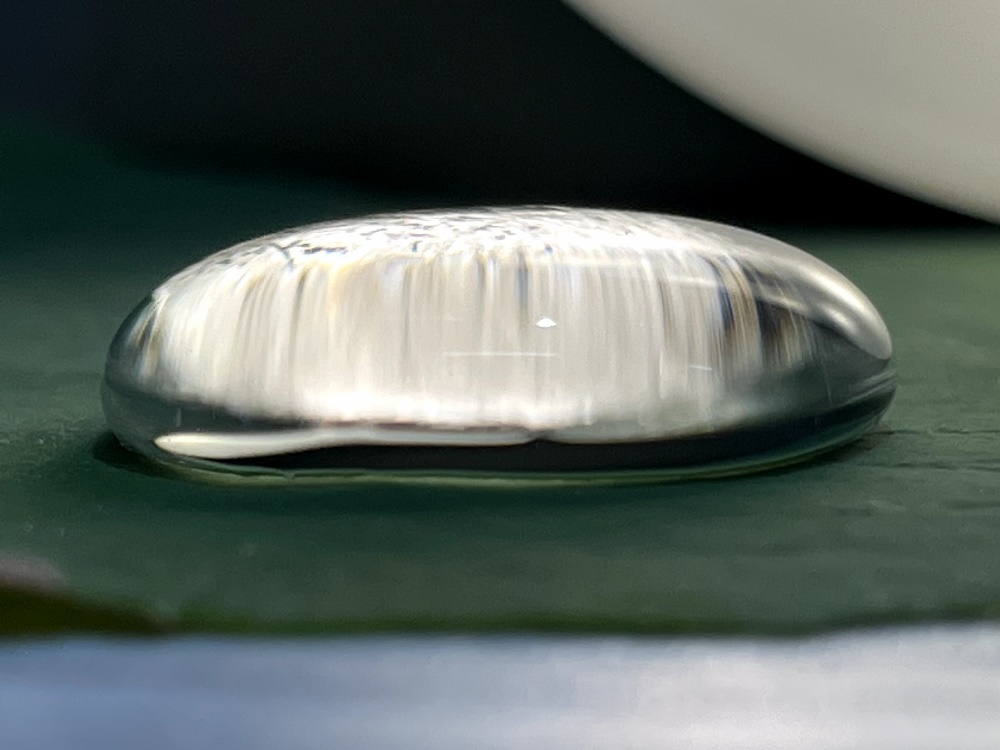
\includegraphics[scale=0.25]{图像/大水滴.png}
        }
    \caption{实验结果}\label{水滴接触角图}
\end{figure}

关于液滴在超疏水表面的形状的描述,会在第\ref{yibanbiaomian}节详细展开. 

\subsubsection{不同极性液体在荷叶表面的状态}
\begin{figure}[H]
    \centering
    \subfigure[状态对比图]{\label{00001}
        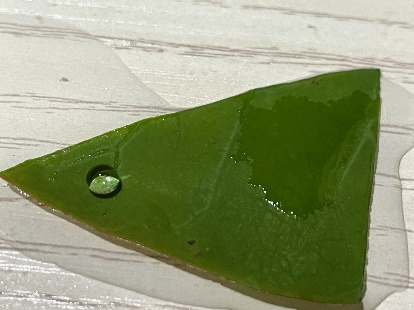
\includegraphics[scale=0.75]{图像/对比图.png}
        }
    \quad
    \subfigure[酒精在荷叶表面的状态]{\label{00002}
        \includegraphics[scale=0.025]{图像/酒精荷叶.png}
        }
    \quad
    \subfigure[晾干后]{\label{00003}
        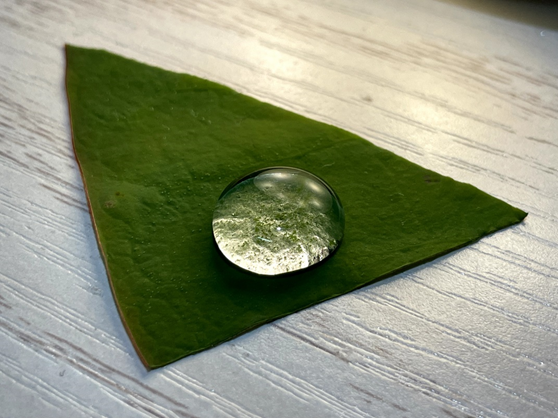
\includegraphics[scale=0.3]{图像/晾干.png}
        }
    \quad
    \subfigure[香油在荷叶表面的状态]{\label{00004}
        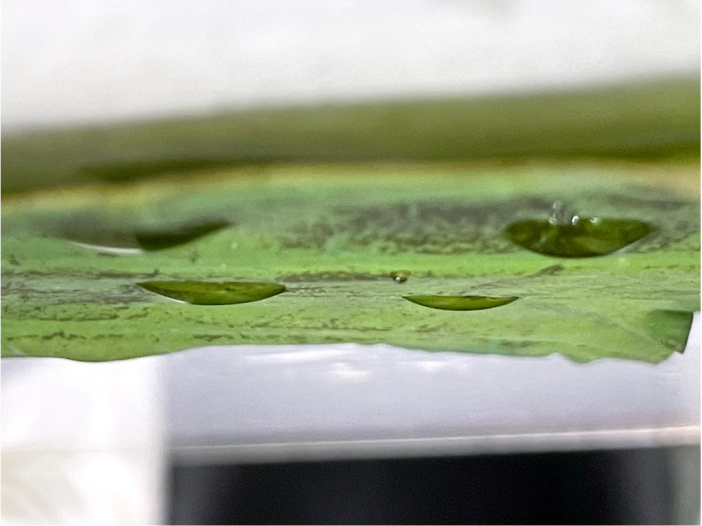
\includegraphics[scale=0.135]{图像/香油.png}
        }
    \caption{实验结果}
\end{figure}
\begin{spacing}{1.528}%段落行距设置
如图\ref{00001}、图\ref{00002}所示,酒精和水两种液滴在荷叶表面的状态差异十分显著,可以看到酒精在其表面完全展平. 
当表面的酒精挥发后,在原本的位置滴加水,仍然呈现出超疏水性,如图\ref{00003}所示,
说明酒精未能破坏荷叶表面的显微结构. 
图\ref{00004}为香油在荷叶表面的状态,可见荷叶无疏油性. 
\end{spacing}

\subsubsection{荷叶滚动角的测量}
\begin{spacing}{1.528}%段落行距设置
搭建如图\ref{10000}所示实验装置,通过缓慢移动垫块来缓慢改变滚动角$\theta$. 在斜面与桌面接触点使用量角器测量滚动角$\theta$. 
与此同时,使用两台设备同时拍摄荷叶上水珠的状态与量角器所示的角度. 
\end{spacing}

\begin{figure}[H]
    \centering
    \subfigure[实验装置]{\label{10000}
        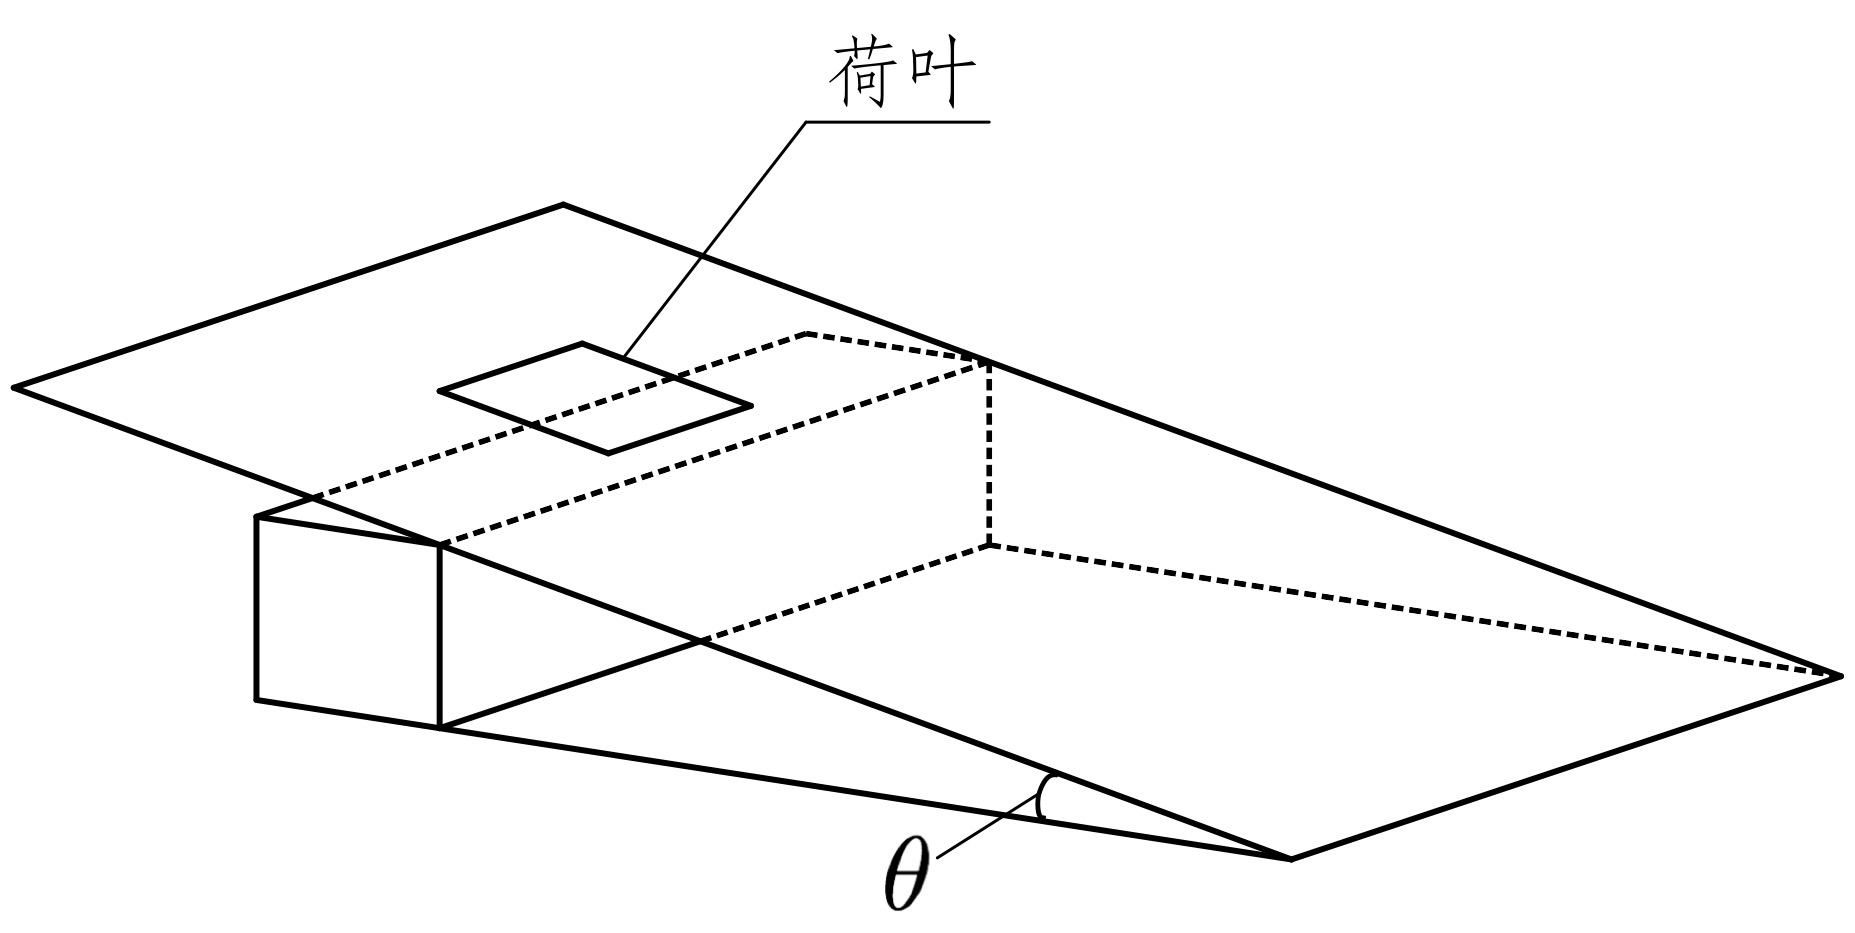
\includegraphics[scale=0.07]{图像/滚动角装置.jpg}
        }
    \quad
    \subfigure[右侧液滴滚动时的滚动角]{\label{10001}
        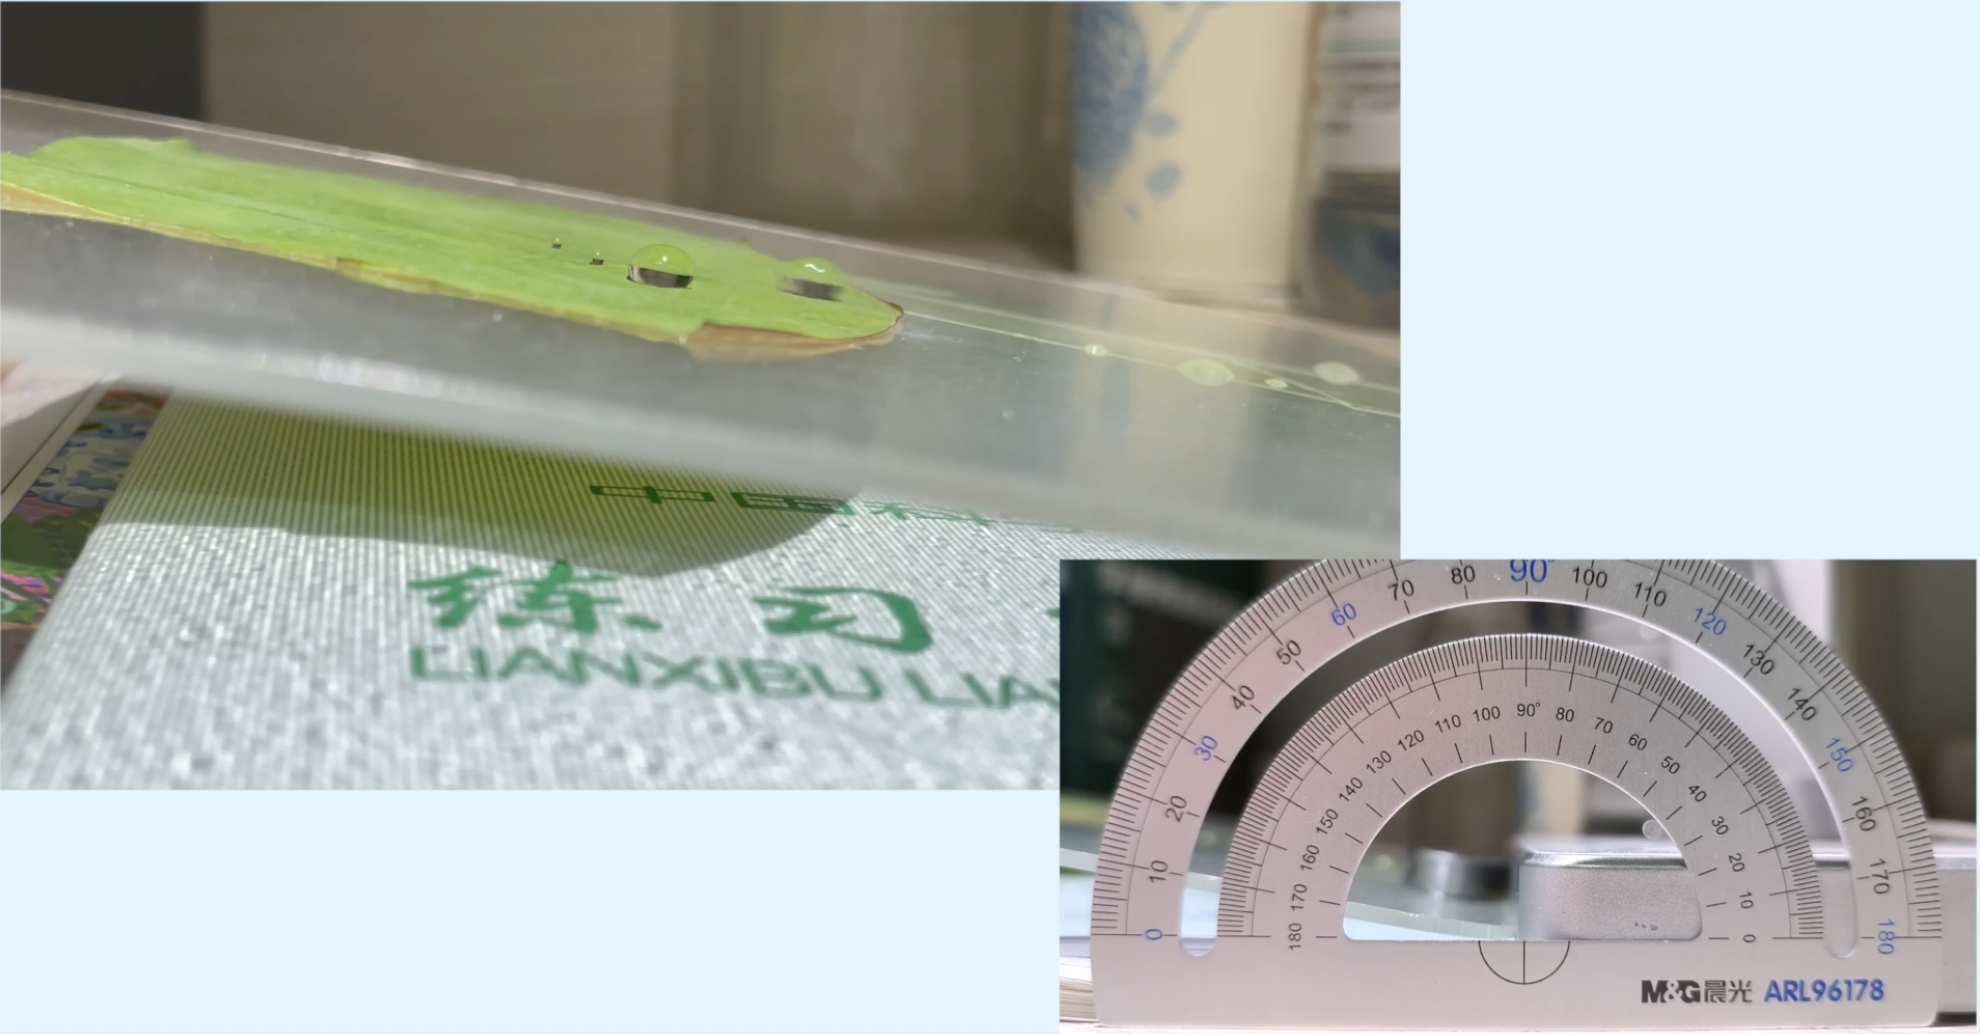
\includegraphics[scale=0.12]{图像/滚动角.png}
        }
    \quad
    \subfigure[悬垂液滴所处的状态]{\label{10002}
        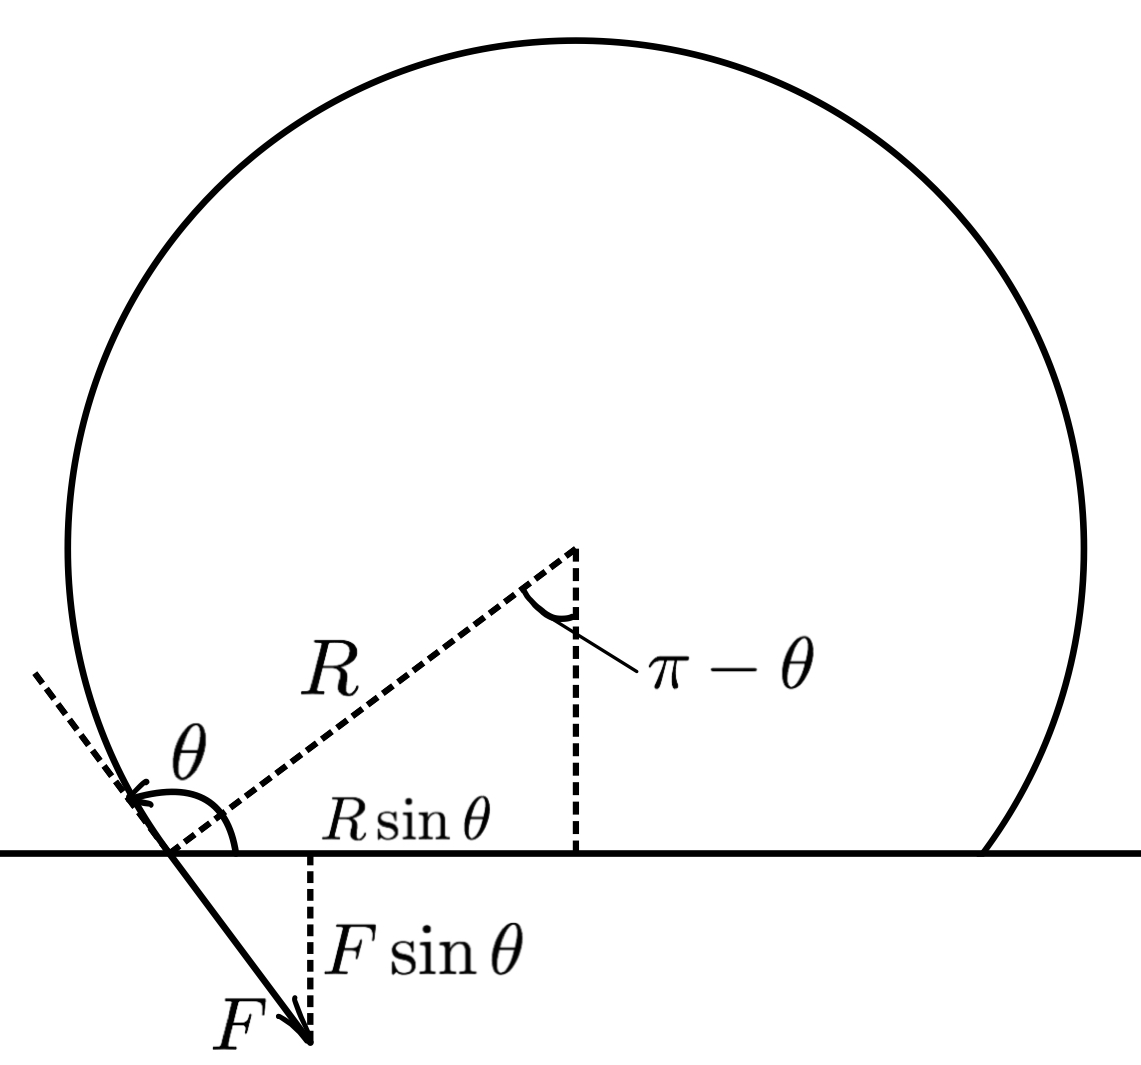
\includegraphics[scale=0.1]{图像/液滴悬垂.jpg}
        }
    \caption{实验结果}
\end{figure}

\begin{spacing}{1.528}%段落行距设置
根据实验测量,可知滚动角约为10\degree,如图\ref{10002}所示,小于超疏水表面定义中的20\degree,因此荷叶表面为超疏水表面. 

值得一提的是,测量滚动角时,最初为了减弱重力的影响,使用的液滴体积尽可能小. 
但是观察到当液滴过小时,测量的滚动角极大,甚至于在荷叶倒置时,水滴仍能悬垂,而不会滴落. 

液滴体积很小时,近似认为是球体,如图\ref{10002}所示. 
可能的原因在于水滴在荷叶表面受到三相点的张力为$2\pi R\sin \theta \gamma \sin \theta =2\pi R\gamma \sin ^2 \theta $,其中$\theta$为接触角,是一个定值. 
而液滴所受重力为$mg=\rho g V=\frac{4}{3}\rho \pi R^3 g$随着$R$的增加,一开始重力小于张力,后来重力大于张力. 
由此较小的液滴会悬而不落,而较大的液滴会滚动与滴落. 
因此最后选择体积较大的液滴以测量滚动角. 
\end{spacing}

\subsubsection{荷叶表面水滴所处状态随时间的的变化}
\begin{spacing}{1.528}%段落行距设置
将水滴通过细管道滴加到荷叶表面后,每日拍摄一次液滴在荷叶上的形状. 
拍摄的照片用Getdata Graph Digitalizer软件处理,手动提取边缘点. 
\end{spacing}
\begin{figure}[H]
    \centering
    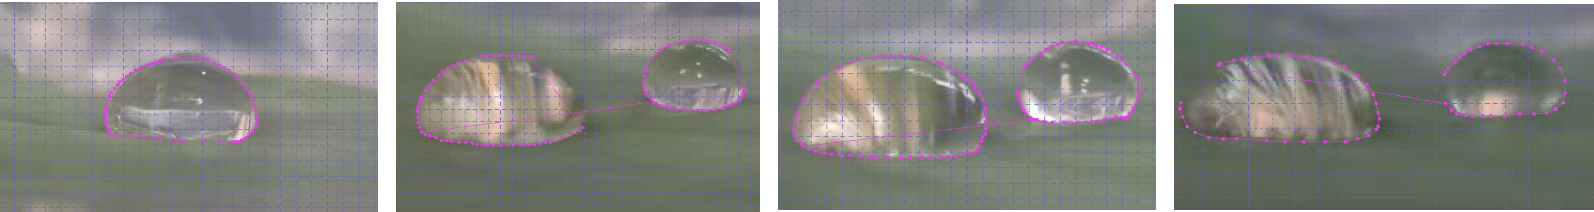
\includegraphics[scale=0.3]{图像/变化.png}
    \caption{几天中荷叶表面液滴形状的变化}\label{12315}
\end{figure}
如图\ref{12315}所示,可以看到水珠在较长时间内形态未发生明显变化. 

\subsubsection{荷叶表面的自清洁现象}
\begin{spacing}{1.528}%段落行距设置
实验装置与测量滚动角时一致,如图\ref{自清洁现象}所示. 在荷叶表面撒上粉末状的某药品,以模拟荷叶表面的污秽物. 向荷叶表面倾洒水,观察在水的作用下荷叶的自清洁性. 
通过实验可以观察到水滴所过之处,药品粉末上留下了一条非常干净的通路. 
\end{spacing}
\begin{figure}[H]
    \centering
    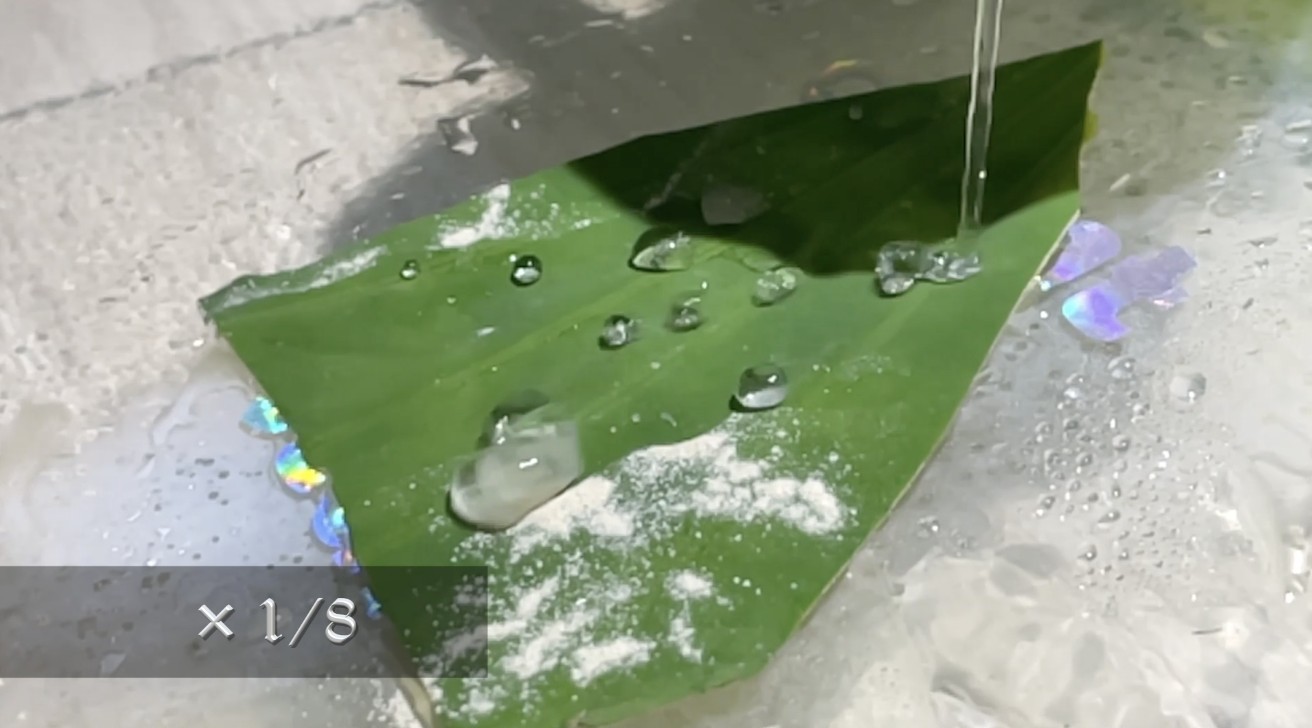
\includegraphics[scale=0.3]{图像/自清洁.png}
    \caption{荷叶的自清洁效应}\label{自清洁现象}
\end{figure}

\subsubsection{水滴在荷叶表面的撞击现象}
在相同高度持续滴落不同大小的水滴于荷叶表面,并使用240fps帧率进行拍摄. 
\begin{figure}[H]
    \centering
    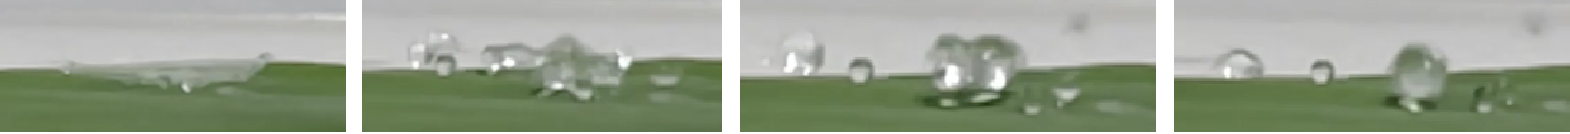
\includegraphics[scale=0.27]{图像/撞击.png}
    \caption{水滴撞击荷叶表面的现象}\label{撞击现象}
\end{figure}

\begin{spacing}{1.528}%段落行距设置
如图\ref{撞击现象}所示,可以观察到,小体积的液滴在撞击荷叶表面后,会基本保持原样弹起,在荷叶表面反复弹跳直至能量耗尽. 
中等体积的液滴会表现出更加明显的弹跳现象,先变为较扁的液滴,而后摊开的液滴迅速收回,整个液滴又会弹起,在荷叶表面重复上述行为直至能量耗尽. 
而大体积的液滴在撞击荷叶表面后,会变得极度扁平,同时边缘会迅速分裂出中、小液滴,向四周射出;而后中小液滴状态如上所述,中央大液滴再度向中收缩、起跳,并重复前述行为. 

出现这种现象的原因可能是液滴在撞击荷叶表面后,下表面液体迅速反弹,而上表面的液体仍以原速下落,内部液体下落过程中多余的动能由于上表面液体迅速下落的压迫和下表面荷叶的止动而被迫转化到水平方向,
使得液体获得指向水平面上各个方向的速度. 
体积大的液滴由于其内部液体含量大、上下表面距离远从而速度差大等原因,其四散的能量大. 

小体积的液滴四散的能量极小、速度较慢,液滴的表面张力可以很轻松地维持液滴原状;
中等体积的液滴四散能量大了一些,表面张力虽能维持液滴不碎裂,但液滴的变形较为明显. 
大水滴四散能量极大,在撞击发生的一瞬间,水的表面张力来不及以维持水滴的形状,于是大液滴便分裂成中、在荷叶表面四散开来. 
\end{spacing}

\subsection{对于一般疏水表面性质的探究}\label{yibanbiaomian}
\subsubsection{理论推导}
根据$\mathfrak{Section}~\uppercase\expandafter{\romannumeral2}$中\ref{adsa}节的推演,给出了水滴形状的控制方程,即一个常微分方程组
$^\text{\cite{ref25,ref26}}$
\begin{equation}\label{ctrleq}
    \left\{
        \begin{aligned}
            &\frac{\text dx}{\text ds}=\cos\theta\\%"&"是对齐位置,即相当于tab. 开头一个&使得公式左对齐
            &\frac{\text dz}{\text ds}=\sin\theta\\%用“\\”换行
            &\frac{\text d\theta}{\text ds}=\frac{2}{r}+cz-\frac{\sin\theta}{x}\\
            &\frac{\text dV}{\text ds}=\pi x^2\sin\theta\\
            &\frac{\text dA}{\text ds}=2\pi x
        \end{aligned}
    \right.
\end{equation}
初始条件为
\begin{equation}
    x(0)=z(0)=\theta(0)=V(0)=A(0)=0\label{zero}
\end{equation}
\begin{spacing}{1.528}%段落行距设置
控制方程\eqref{ctrleq}中,$r$为液滴顶部的曲率半径,$c=\frac{\rho g}{\gamma}$,$V$表示液滴体积,$A$表示液滴截面积. 
\\\suo 值得注意的是,当$s=0$时,控制方程\eqref{ctrleq}中第三式将会出现奇异性,化简后的形式为
\begin{equation}
    \frac{\text d\theta}{\text ds}=\frac{1}{r}\label{zzero}
\end{equation}
这样式\eqref{ctrleq}\eqref{zero}\eqref{zzero}构成一个常微分方程组,通过给合适的初值$s,r$,便可求出控制方程的数值解,将其中$z-x$图作出,即为ADSA的结果,也就是对液滴形状的预测. 
\\\suo 那么问题就来到了如何获得恰当的$s$与$r$值. 事实上,可以通过给一个合适的初值$s_0,r_0$求解控制方程的数值解,获得$\theta$与$V$的值,与实验数据$\theta_e,V_e$做比较,然后便可通过通过牛顿迭代法或二分法来逼近$s,r$的真实值
$^\text{\cite{ref27,ref28,ref29,ref30,ref31}}$. 
误差范围内,便可以代入上一段所述方法,画出最贴近于现实的预测图像. 
\\\suo 课题组使用了Matlab来完成这一过程(附录). 以$\theta_e = 117.34\degree,V_e = 8.92\times10^{-8}\text m^3$为例,可以看到,在第二次逼近后,相对误差已经下降到$0.5\%$以下(附录)(图\ref{V}). 
\end{spacing}
\begin{figure}[H]
    \centering
    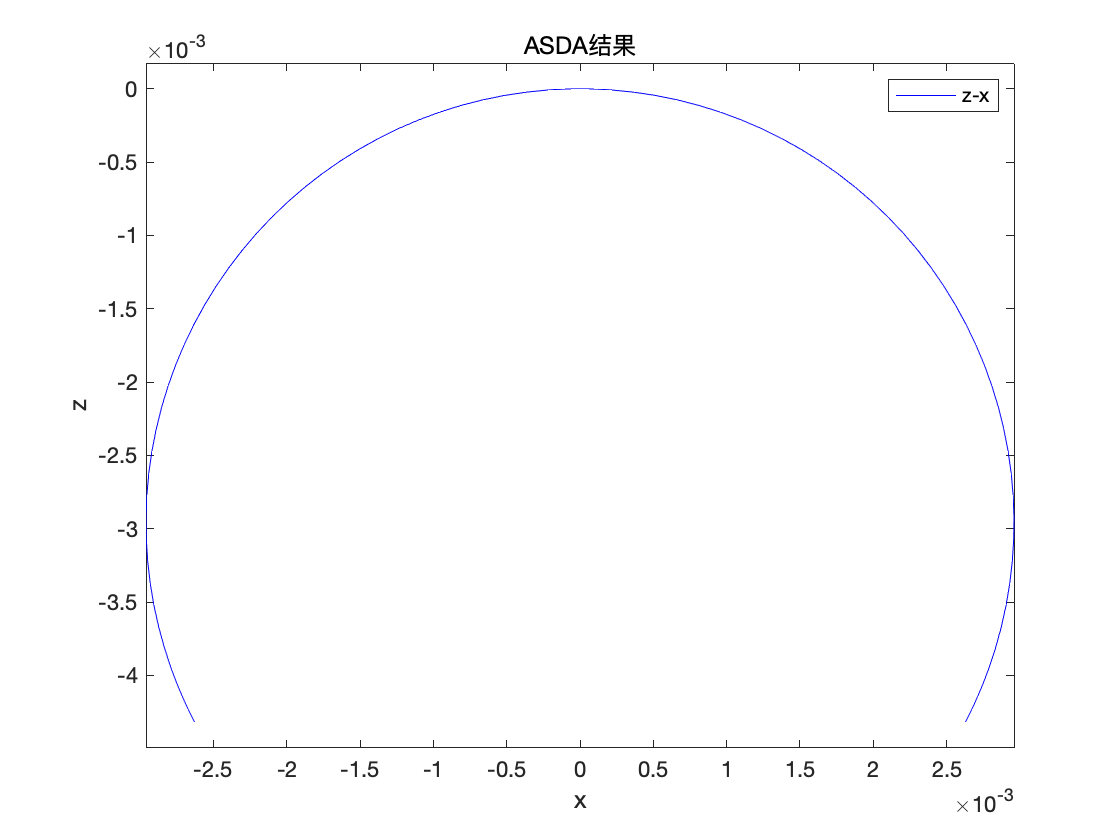
\includegraphics[scale=0.15]{图像/V=8.92e-8.png}
    \caption{ADSA结果(单位:m)}\label{V}
\end{figure}

\subsubsection{实验方法与过程}
在实验部分,使用专用摄像机与强光源,对不同液滴在不同表面上的不同状态进行了拍摄. 
\begin{figure}[H]
    \centering
    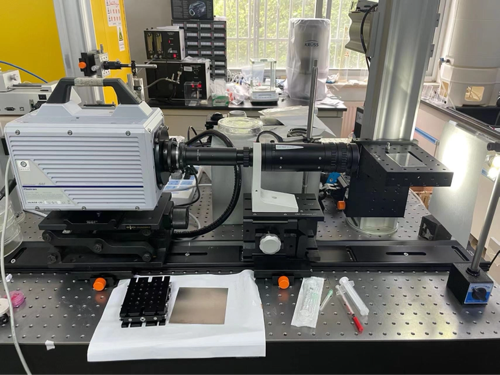
\includegraphics[scale=0.4]{图像/实验装置.png}
    \caption{实验装置}
\end{figure}

\subsubsection{实验结果与数据处理}
以下(图\ref{实验})为摄像机拍摄到的图像:
\begin{figure}[H]
    \centering
    \subfigure[纯水-1700电子镀膜剂涂层玻璃]{
        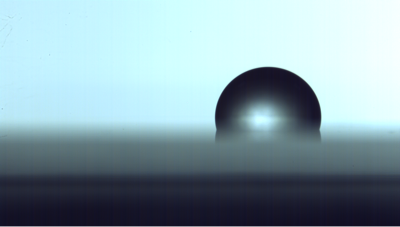
\includegraphics[scale=0.25]{图像/1700水实验.png}
        }
    \quad
    \subfigure[5cst硅油-1700电子镀膜剂涂层玻璃]{
        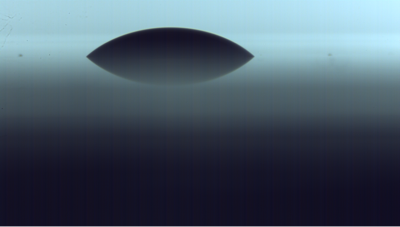
\includegraphics[scale=0.25]{图像/1700硅油实验.png}
        }
    \quad
    \subfigure[纯水-Glaco涂层玻璃]{
        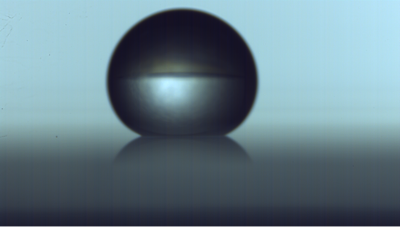
\includegraphics[scale=0.25]{图像/glaco水实验.png}
        }
    \quad
    \subfigure[5cst硅油-Glaco涂层玻璃]{\label{glaco硅油}
        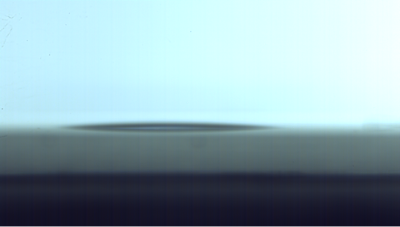
\includegraphics[scale=0.25]{图像/glaco硅油实验.png}
        }
    \caption{实验结果}\label{实验}
\end{figure}
用现场的计算机测得接触角如下表\ref{接触角表}:
\begin{table}[H]
    \begin{center}
        \caption{接触角}\label{接触角表}
        \begin{tabular}{cc}
            \toprule
            类型 & 接触角(\degree)\\
            \midrule
            纯水-1700电子镀膜剂涂层玻璃&105.64\\
            5cst硅油-1700电子镀膜剂涂层玻璃&37.21\\
            纯水-Glaco涂层玻璃&157.00\\
            \bottomrule
        \end{tabular}
    \end{center}
\end{table}
\begin{spacing}{1.528}%段落行距设置
不难看出,图\ref{glaco硅油}所示5cst硅油-Glaco涂层玻璃中接触角过小,浸润程度非常大,此法难以对其进行分析,故不再继续处理. 
对上述图片(图\ref{实验})进行色彩处理得图\ref{色彩}:
\end{spacing}
\begin{figure}[H]
    \centering
    \subfigure[纯水-1700电子镀膜剂涂层玻璃]{
        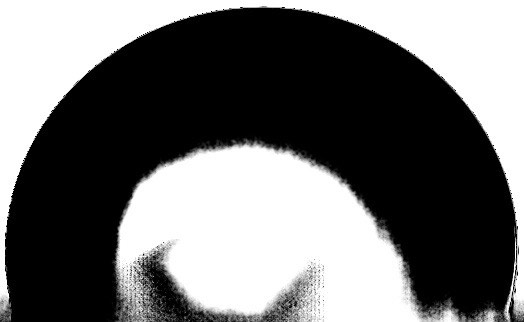
\includegraphics[scale=0.125]{图像/1700水处理.png}
        }
    \quad
    \subfigure[5cst硅油-1700电子镀膜剂涂层玻璃]{
        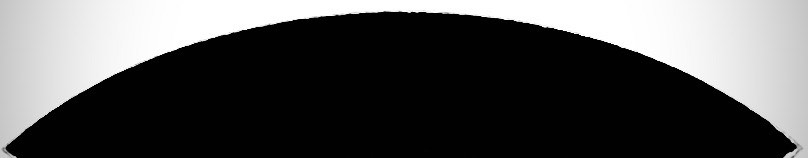
\includegraphics[scale=0.125]{图像/1700硅油处理.png}
        }
    \quad
    \subfigure[纯水-Glaco涂层玻璃]{
        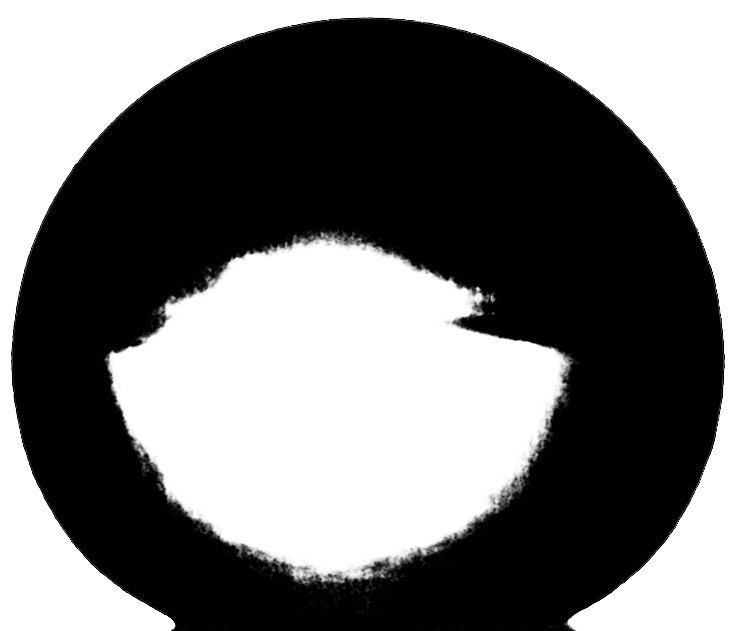
\includegraphics[scale=0.125]{图像/glaco水处理.png}
        }
    \caption{色彩处理}\label{色彩}
\end{figure}
用Matlab提取边界可得图\ref{边缘}:
\begin{figure}[H]
    \centering
    \subfigure[纯水-1700电子镀膜剂涂层玻璃]{
        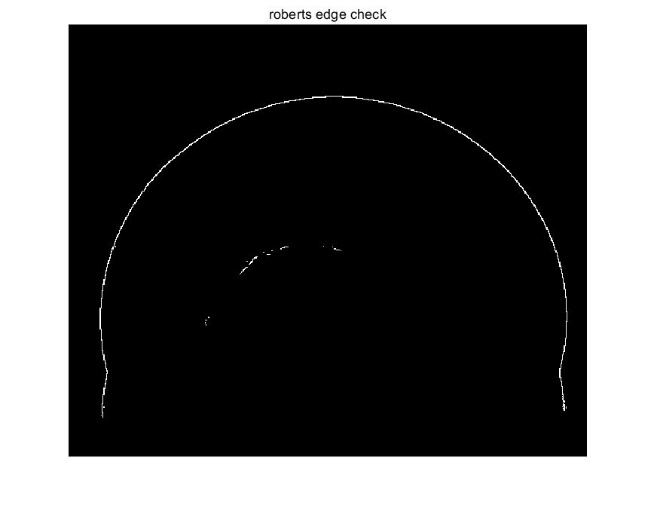
\includegraphics[scale=0.5]{图像/1700水边缘.png}
        }
    \quad
    \subfigure[5cst硅油-1700电子镀膜剂涂层玻璃]{
        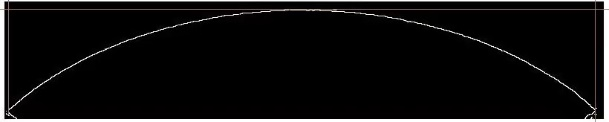
\includegraphics[scale=0.5]{图像/1700硅油边缘.png}
        }
    \quad
    \subfigure[纯水-Glaco涂层玻璃]{
        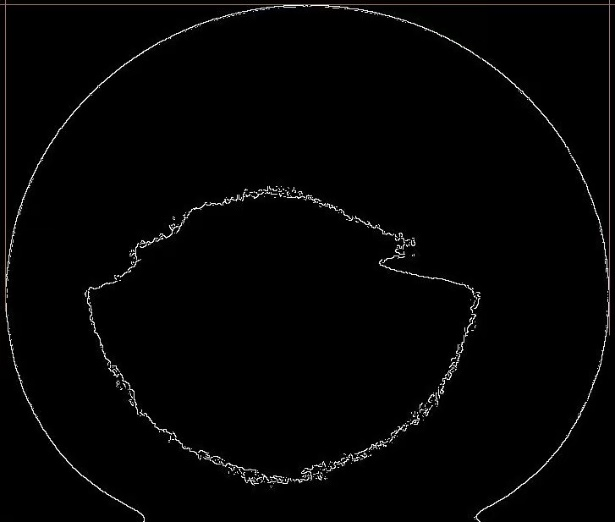
\includegraphics[scale=0.5]{图像/glaco水边缘.png}
        }
    \caption{提取边缘}\label{边缘}
\end{figure}
最后用GetData提取边界的数据点如图\ref{数据}:
\begin{figure}[H]
    \centering
    \subfigure[纯水-1700电子镀膜剂涂层玻璃]{
        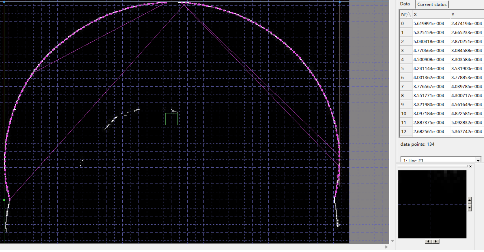
\includegraphics[scale=0.25]{图像/1700水数据.png}
        }
    \quad
    \subfigure[5cst硅油-1700电子镀膜剂涂层玻璃]{
        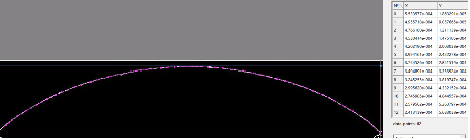
\includegraphics[scale=0.25]{图像/1700硅油数据.png}
        }
    \quad
    \subfigure[纯水-Glaco涂层玻璃]{
        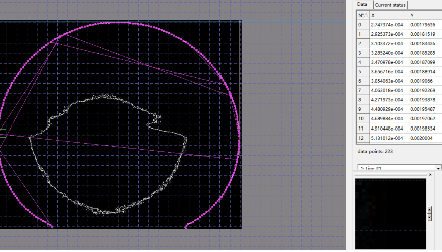
\includegraphics[scale=0.25]{图像/glaco水数据.png}
        }
    \caption{提取数据点}\label{数据}
\end{figure}
至此,图片所能提供的信息已被提取完毕. 
\begin{figure}[H]
    \centering
    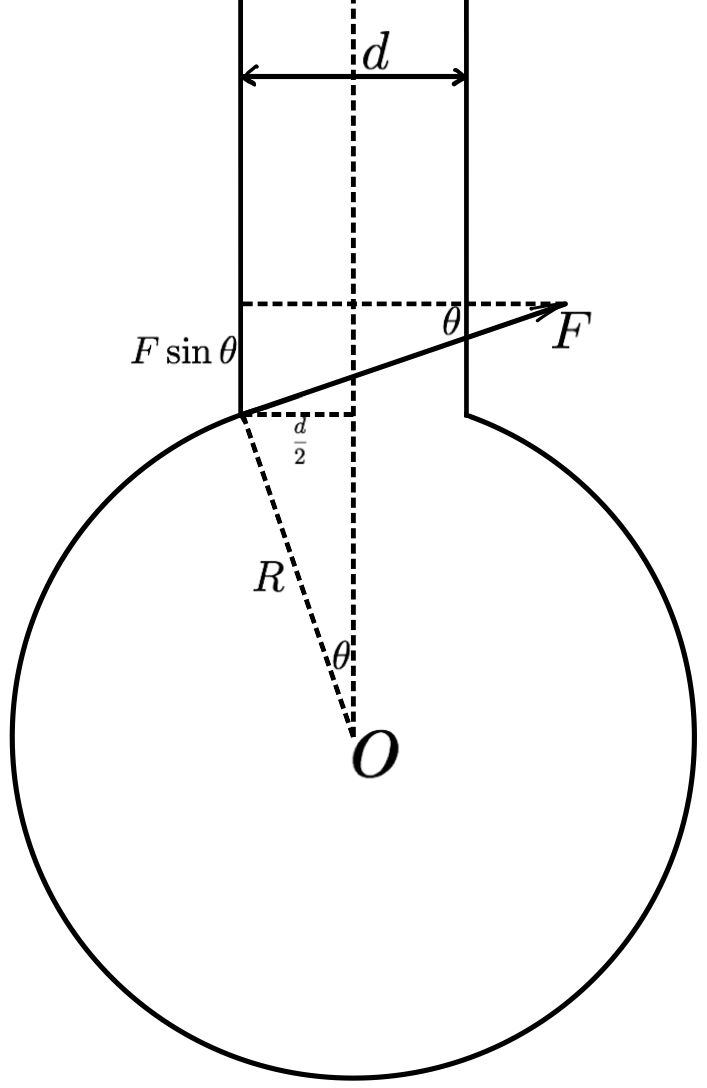
\includegraphics[scale=0.2]{图像/毛细管.jpg}
    \caption{毛细管悬垂的水滴体积}\label{96178}
\end{figure}
对于液滴体积的测量,如图\ref{96178}所示,由于液滴是通过毛细管滴下,因此有
\begin{equation}
    2\pi  \frac{d}{2} \gamma\sin \theta=2\pi  \frac{d}{2}\gamma\frac{d/2}{R}=\rho gV=\rho g \frac{4}{3}\pi R^3 \label{液滴体积}
\end{equation}
\begin{spacing}{1.528}%段落行距设置
已知毛细管直径$d=3.3\times 10^{-4}~$m,则由式(\ref{液滴体积})可求出液滴半径$R_\text{纯水}=7.426\times 10^{-4}~$m,$R_\text{硅油}=5.818\times 10^{-4}~$m
因此液滴体积$V_\text{纯水}=1.715\times 10^{-9}~\text{m}^3$,$V_\text{硅油}=8.251\times 10^{-10}~\text{m}^3$. 
\\\suo 将这些数据代入附录所示程序中,可得理论预计的边界曲线与实际曲线的形状如图\ref{最终结果}(红线为模拟结果,蓝点为通过上述过程提取出的数据点):
\end{spacing}
\begin{figure}[H]
    \centering
    \subfigure[纯水-1700电子镀膜剂涂层玻璃]{
        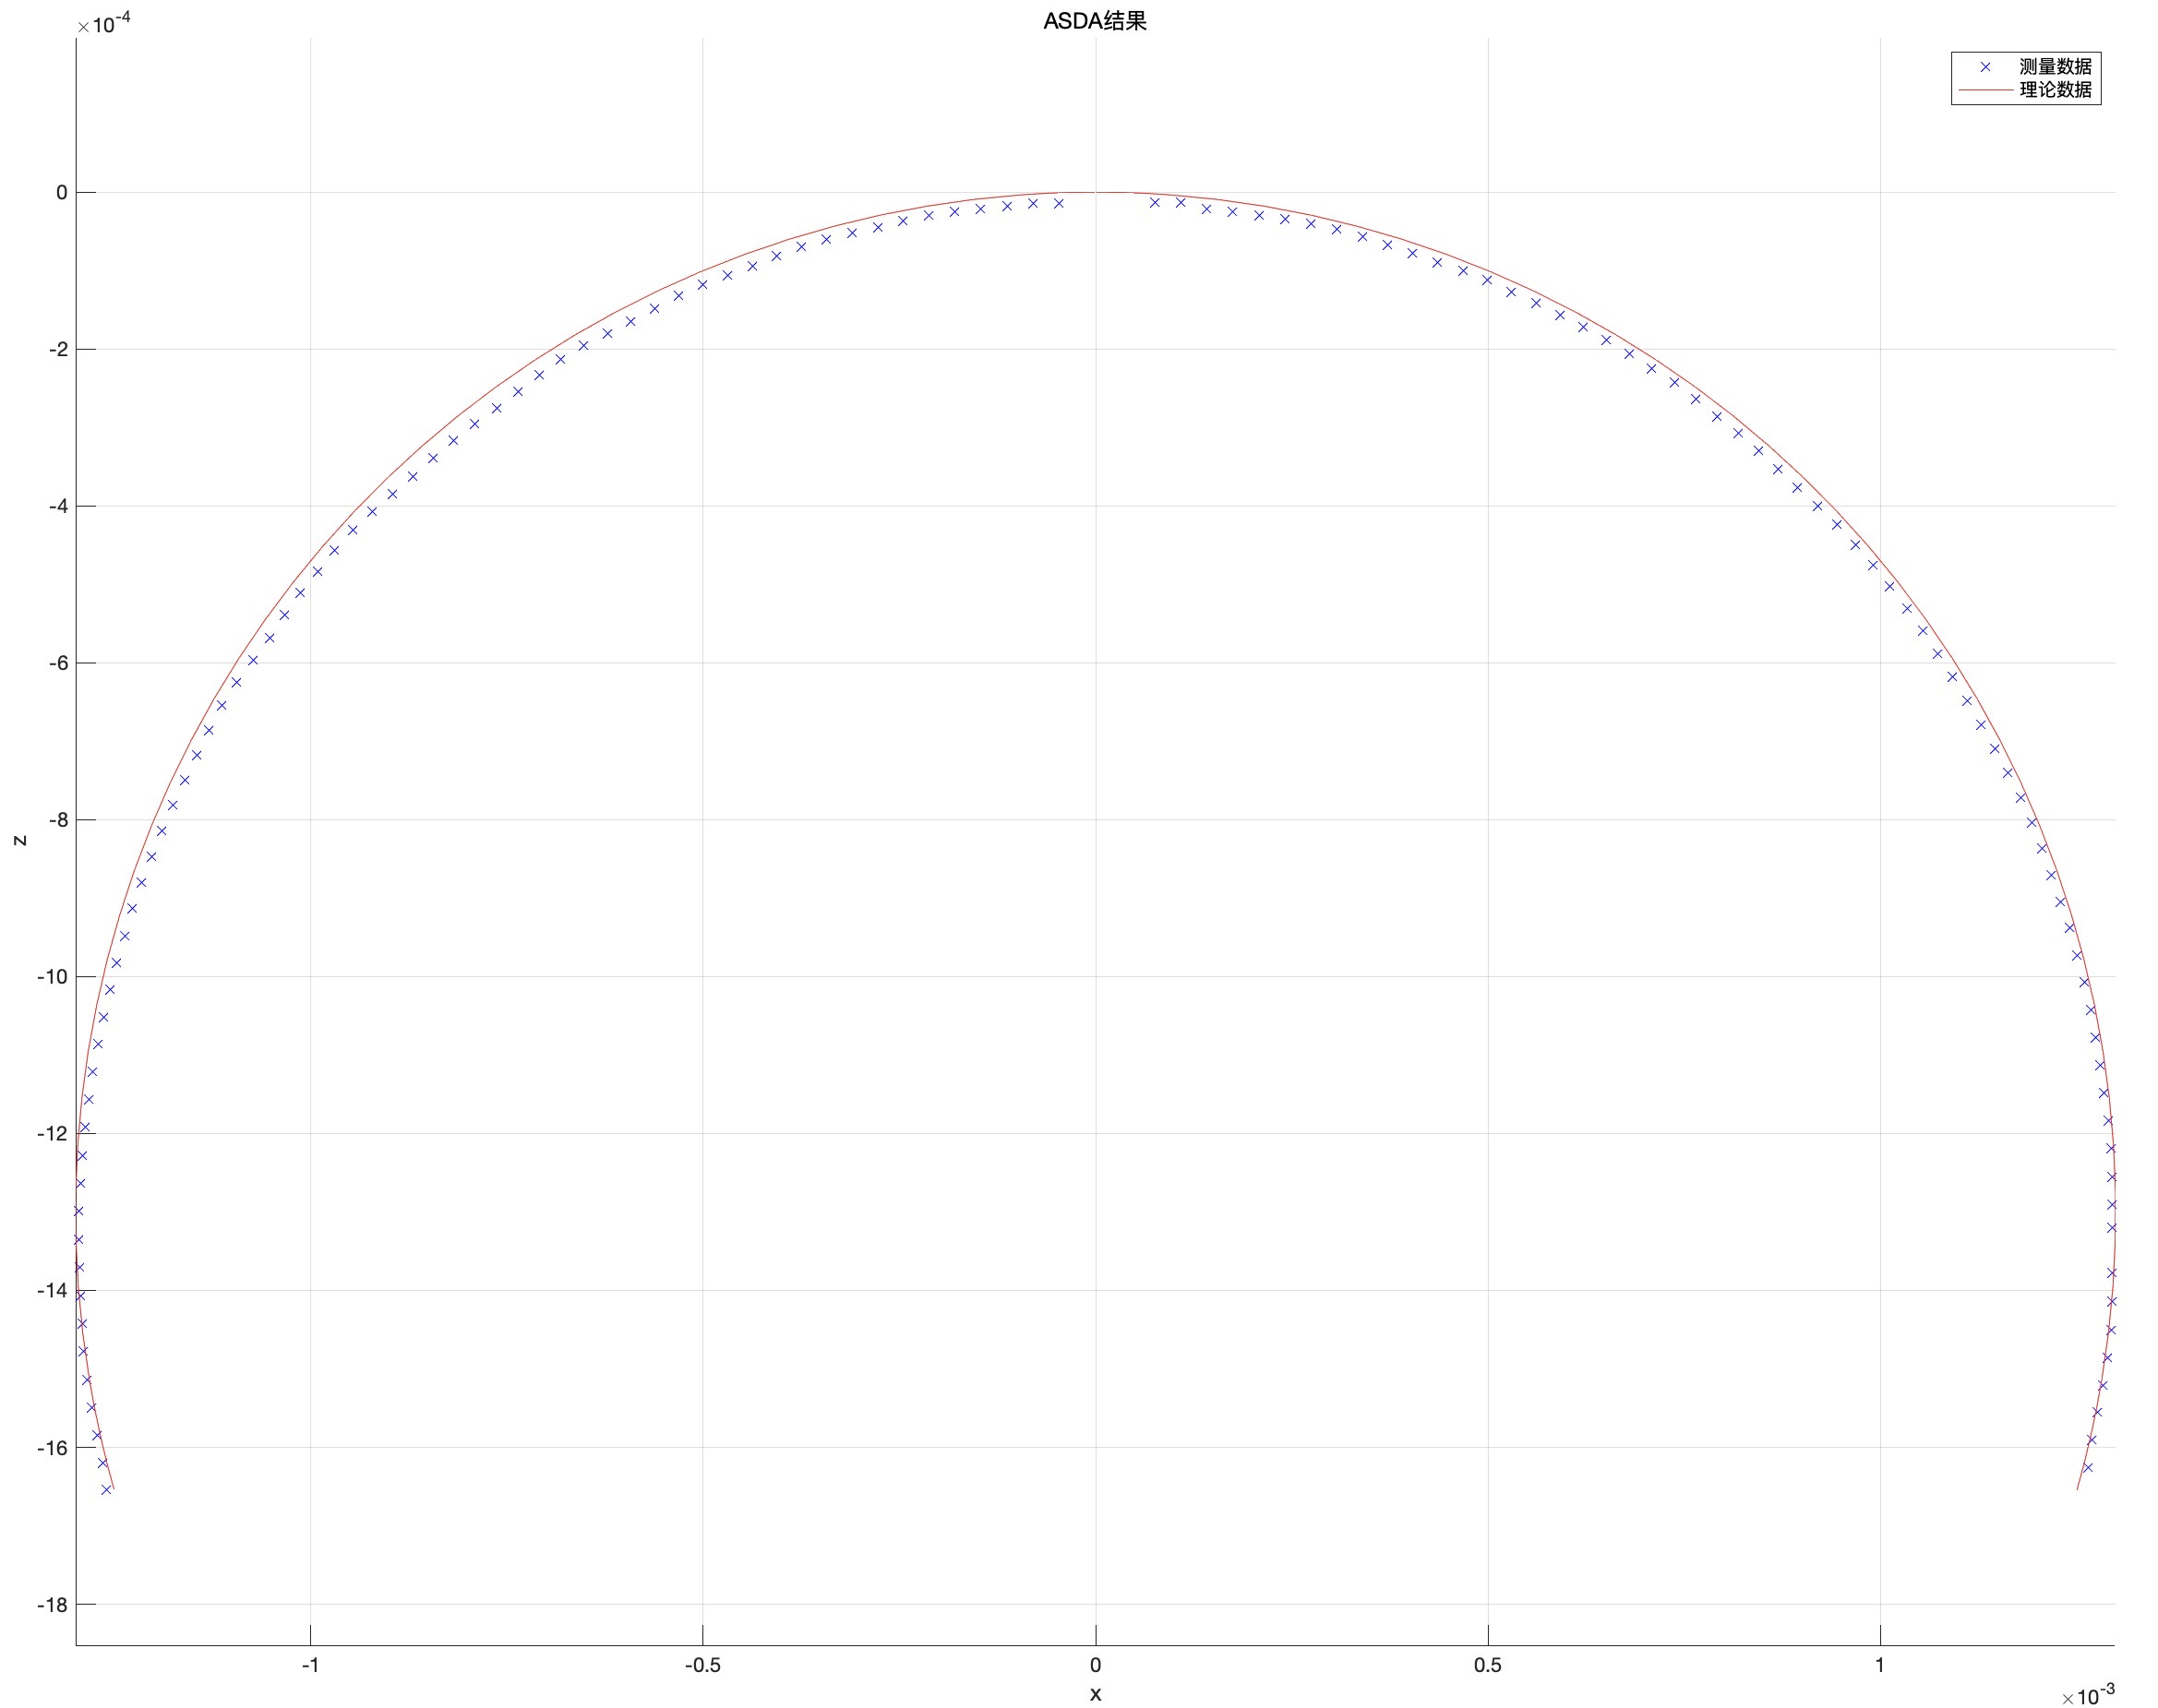
\includegraphics[scale=0.06]{图像/1700水结果.jpeg}
        }
    \quad
    \subfigure[5cst硅油-1700电子镀膜剂涂层玻璃]{
        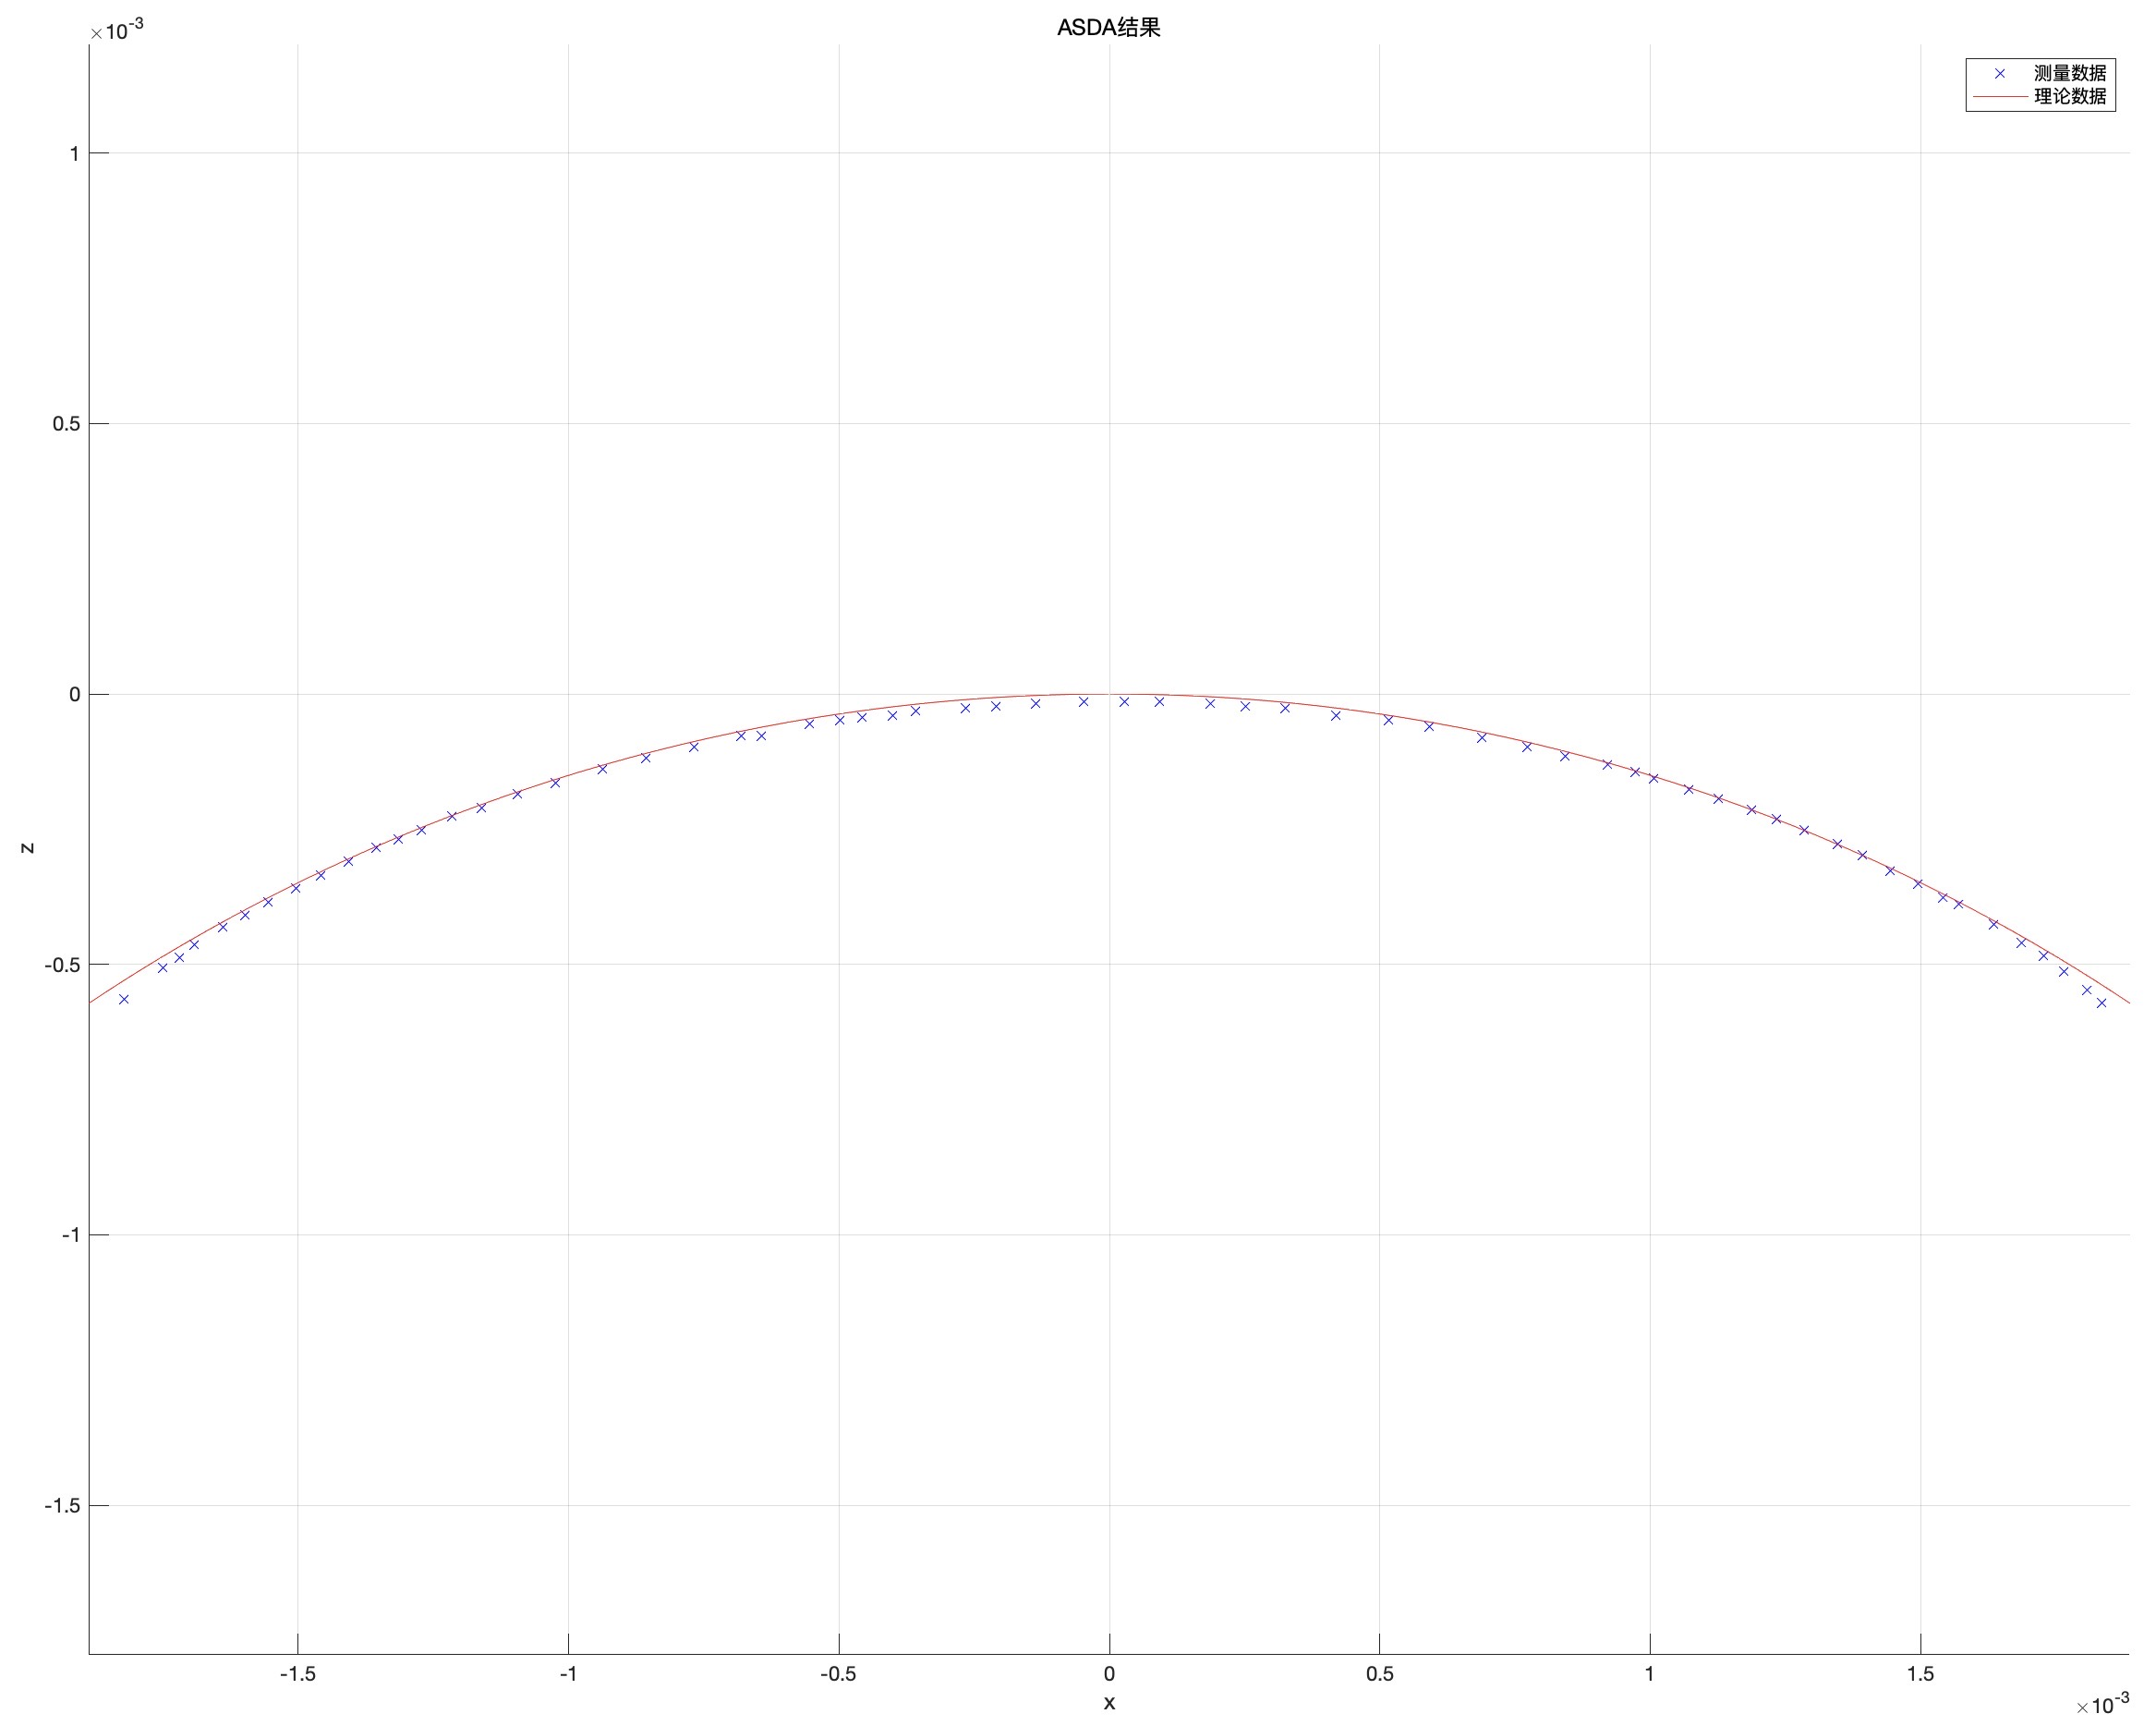
\includegraphics[scale=0.06]{图像/1700硅油结果.jpeg}
        }
    \quad
    \subfigure[纯水-Glaco涂层玻璃]{
        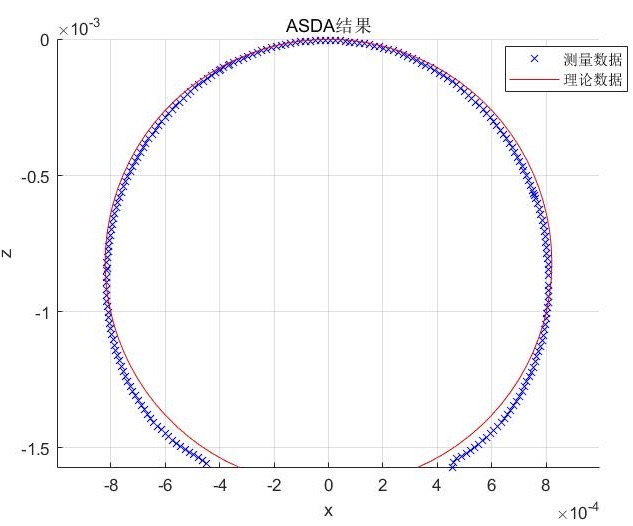
\includegraphics[scale=0.2]{图像/glaco水结果.jpeg}
        }
    \caption{ADSA结果(单位:m)}\label{最终结果}
\end{figure}

\subsubsection{讨论}
在实践中发现,如果$V$与$\theta$输入值有小偏差,则最终结果会相差甚远. 

\section{结论}
%不仅阐述研究过程得出了怎样的结论,在第三章中提的假设到底哪些成立哪些不成立
%而且关系到研究成果或论文的成果到底有什么意义,有没有实用价值. 
\begin{spacing}{1.528}%段落行距设置
\begin{enumerate}
    \item 荷叶具有超疏水性与自清洁性,无疏油性;
    \item 荷叶具有乳突等微结构,产生了疏水能力;
    \item 误差产生的原因:
    对$\theta$和$V$的实验值,需要较高精度,否则不会收敛到打靶用实验值;
    $\theta$和$V$即使遍历范围小,在小范围内形状变化也可以很大;
    对于给定$\theta$和$V$求出的解没有唯一性. 
\end{enumerate}
\end{spacing}
%\end{multicols}%结束分栏

\section{结语}%不足与展望
%挑几个不那么原则性的问题说一说,比如:调研对象范围不够广,理论模型可以再细化等等……
%希望后人可以继续研究等简单展望一下. 
\begin{spacing}{1.528}%段落行距设置
本课题系统探究了荷叶及其他疏水表面的性质,对相关理论进行了学习与探讨,并提出了相关见解;但还存在一些不足之处,
比如调研的对象——即其他疏水表面——的种类还不够多,只调研了两种表面,且液体也只选用了纯水和硅油两种液体;
再比如ADSA的理论模型还能够再细化,但碍于课题组的学业水平,未能取得较为深刻的进展,等等. 
希望后续的研究者能够借鉴本课题的成果与不足,拓展研究面,细化理论模型,改进求解算法,进而取得更加深入的突破. 
\end{spacing}

\section{致谢}%致谢
%致谢
\begin{spacing}{1.528}%段落行距设置
大学生活中第一次做课题,做了大一一整个学年,如今终于完成,心中感慨万千. 

首先要感谢本门课的授课教师高鹏老师. 高老师为人十分和蔼、平易近人,对学术非常认真,对学生也非常照顾. 
高老师带领着刚进入大学的我们学会了如何做一个简单的课题,在我们学术研究方面是启蒙教师,居功至伟. 

另外要感谢组内所有的同学,感谢同学的陪伴、支持与帮助. 

然后要感谢近代力学系高速界面流动实验室的研究生学长邵政豪,他带领我们测量了各种液滴在不同表面的接触角,在我们的实验与数据测量中功不可没,
并为我们拓展研究面提供了宝贵的意见和建议. 

还要感谢曾经给予我们指导的老师们,有我们的班主任吴尚犬老师,教我们力学的王海龙老师,教授物理化学课程的汪文栋老师等. 
感谢老师们的指导,为我们完成课题做出了巨大贡献,让我们成长. 

接着要感谢我们的室友们,为我们提供了很多重要的新颖的思路与见解. 

以及要感谢互联网上不知名的网友们,他们遍布在知乎、CSDN、bilibili、百度知道、百度百科等等等等平台,
他们给我们提供了海量宝贵的资源,让我们得以迅速获取需要的知识. 

最后一定要感谢我们的母校,中国科学技术大学,是她给我们提供了宝贵的平台,使我们
在使用知网、Matlab等时并未遭到资本家的剥削与压迫,等等等等. 

感谢所有帮助过我们的个人、机构、组织!感谢我们伟大的祖国——中国!

\rightline{\today}
\end{spacing}

\newpage
\begin{thebibliography}{23}%不使用BibTeX的方法;99意为参考文献的最大数值为99个,这个数可以自己设置
    \bibitem{ref1}百度百科. 莲花效应[DB/OL]. (2021-12-05)[2022-02-23]. https://baike.baidu.com/item/莲花效应/3702289.
    \bibitem{ref2}刘双平, 俞熹. 荷叶效应的研究[J]. 大学物理, 2011, 30(9): 50-50.
    \bibitem{ref3}赵宁, 卢晓英, 张晓艳, 等. 超疏水表面的研究进展[J]. 化学进展, 2007, 19(06): 860.
    \bibitem{ref4}李国滨, 刘海峰, 李金辉, 等. 超疏水材料的研究进展[J]. 高分子材料科学与工程, 2020, 36(12): 142-150.
    \bibitem{ref5}姜淑慧.荷叶效应及其在仿生学上的应用[J].生物学教学,2013,38(04):62-63+43.
    \bibitem{ref6}王宇捷.荷叶效应及其在生活中的应用[J].当代化工研究,2018(09):122-123.
    \bibitem{ref7}刘啸成,戴礼兴.自清洁材料的现状与发展[J].中国石油和化工标准与质量,2017,37(17):84-85.
    \bibitem{ref7.5}百度百科. 表面张力[DB/OL]. (2022-01-12)[2022-02-25]. https://baike.baidu.com/item/表面张力
    \bibitem{ref8}百度百科. 接触角[DB/OL]. (2021-06-08)[2022-02-24]. https://baike.baidu.com/item/接触角/10858958
    \bibitem{ref9}张博. 液滴润湿行为与表面微纳结构关系的模拟研究[D].北京化工大学,2016.
    \bibitem{ref17}百度百科. 滚动角[DB/OL]. (2022-01-08)[2022-02-24]. https://baike.baidu.com/item/滚动角/3102389
    \bibitem{ref18}X-MOL. 构筑超浸润表面:“玫瑰”向左,“荷叶”向右[EB/OL]. (2018-01-03)[2022-02-24]. https://www.x-mol.com/news/10666\#:~:text=“玫瑰花效应”和,不同的润湿特性.
    \bibitem{ref21}百度百科. 杨-拉普拉斯公式[DB/OL]. (2020-12-08)[2022-02-23]. https://baike.baidu.com/item/杨-拉普拉斯公式/8307652.
    \bibitem{ref22}Saad S M I, \textit{Neumann A W. Axisymmetric drop shape analysis (ADSA): an outline}[J]. Advances in Colloid and Interface Science, 2016, 238: 62-87.
    \bibitem{ref23}宁乔,朱志强,吕旭涛,于强,袁章福.图像法求液滴表面张力和接触角[J].空间科学学报,2008(01):74-79.
    \bibitem{ref24}百度百科. 毛细管数[DB/OL]. (2016-11-16)[2022-02-25]. https://baike.baidu.com/item/毛细管数/5067694
    \bibitem{ref25}知乎. Young-Laplace方程的应用[EB/OL]. (2018-09-10)[2022-03-32]. https://zhuanlan.zhihu.com/p/42473736
    \bibitem{ref26}知乎. Young-Laplace方程的应用2[EB/OL]. (2021-08-29)[2022-03-02]. https://zhuanlan.zhihu.com/p/404600127
    \bibitem{ref27}吕巍, 魏良亭, 冯恩民. 一类求解非线性奇异方程组的牛顿改进算法[J]. 控制与决策, 2017, 12(32): 2240-2246.
    \bibitem{ref28}Kou J, Li Y, Wang X. \textit{Efficient continuation Newton-like method for solving systems of non-linear equations}[J]. Applied mathematics and computation, 2006, 174(2): 846-853.
    \bibitem{ref29}Wu X. \textit{Note on the improvement of Newton’s method for system of nonlinear equations}[J]. Applied Mathematics and Computation, 2007, 189(2): 1476-1479.
    \bibitem{ref30}Hueso J L, Martínez E, Torregrosa J R. \textit{Modified Newton’s method for systems of nonlinear equations with singular Jacobian}[J]. Journal of Computational and Applied Mathematics, 2009, 224(1): 77-83.
    \bibitem{ref31}Wu X Y. \textit{A new continuation Newton-like method and its deformation}[J]. Applied mathematics and computation, 2000, 112(1): 75-78.
\end{thebibliography}

\newpage
\begin{appendices}

\section*{附录~~~Matlab代码及输出结果}\label{code}
    \subsection*{函数文件odefun.m}
    \footnotesize{\setmainfont{Courier New Bold}% 设置代码字体
        %下一行:开始代码区,语言为Matlab
        %%%%%%%%%%重要!!!!!!!!!!!!代码区代码一定要顶格写!!!!!!!tab键会被显示出来!!!!!!!!!!!!!!!!
        \begin{lstlisting}[language=Matlab]
function out = odefun(s,in)
%控制方程
%in(1)==x,in(2)==z,in(3)==theta,in(4)==V,in(5)==A%变量
%in(6)==r,r是参数,不是变量,用这个方法传参

%常数
g = 9.7947;%合肥
rho = 0.997044;%25度
gamma = 0.07197;%25度
c = rho * g / gamma;

%列方程
out = zeros(6,1);
out(1) = cos(in(3));
out(2) = sin(in(3));
if in(1) == 0 %初始条件下控制方程(3)式变为如下形式
    out(3) = 2 / in(6);
else %其他条件下保持原样
    out(3) = 2/in(6) + c*in(2) - (sin(in(3)))/(in(1));
end
out(4) = pi * (in(1)^2) * sin(in(3));
out(5) = 2 * pi * in(1);

end
        \end{lstlisting}
    }

\subsection*{脚本文件main.m}
    {\setmainfont{Courier New Bold}
        \begin{lstlisting}[language=Matlab]
clear
clc
format long

% 输入实验数据
theta_e = deg2rad(117.34);
V_e = 8.92e-8;
x=1e-3;
z=0;
theta=1e-3;
V=0;
A=0;%r1=5e-3;s1 = 5e-3;

% 二分法遍历
for a=1:4
    r1=a/1000;
    for b=1:4
        s1=b/1000;
        tspan = [-s1 s1];
        in0 = [1e-6 0 1e-6 0 0 r1];
        [x,in] = ode45('odefun',tspan,in0);
        theta1 = in(end,3);%取r1时的theta
        V1 = in(end,4);
        theta_cha=theta_e-theta1;
        V1_cha=V_e-V1;
        if a==1 && b==1
            theta_min=theta1;
            V1_min=V1;
            theta_cha1=theta_cha;
            V1_cha1=V1_cha;
            r_min=r1;
            s_min=s1;
        elseif (abs(theta_cha1)-abs(theta_cha))>0 && 
                    abs(V1_cha1)-abs(V1_cha)>0
            theta_min=theta1;
            theta_cha1=theta_cha;
            V1_min=V1;
            V1_cha1=V1_cha;
            r_min=r1;
            s_min=s1;
        end
    end
end
tspan = [-s_min s_min];%求解范围
in0 = [1e-6 0 1e-6 0 0 r_min];%五个的初值,以及常数r
[x,in] = ode45('odefun',tspan,in0);
%解方程,数值解存入x,y中

% 第二次遍历
theta_e = deg2rad(117.34);
V_e = 8.92e-8;
x=1e-3;
z=0;
theta=1e-3;
V=0;
A=0;%r1=5e-3;s1 = 5e-3;

for a=200:400
    r1=a/100000;
    for b=200:400
        s1=b/100000;
        tspan = [-s1 s1];
        in0 = [1e-6 0 1e-6 0 0 r1];
        [x,in] = ode45('odefun',tspan,in0);
        theta1 = in(end,3);%取r1时的theta
        V1 = in(end,4);
        theta_cha=theta_e-theta1;
        V1_cha=V_e-V1;
        if a==1 && b==1
            theta_min=theta1;
            V1_min=V1;
            theta_cha1=theta_cha;
            V1_cha1=V1_cha;
            r_min=r1;
            s_min=s1;
        elseif (abs(theta_cha1)-abs(theta_cha))>0 && 
                    abs(V1_cha1)-abs(V1_cha)>0
            theta_min=theta1;
            theta_cha1=theta_cha;
            V1_min=V1;
            V1_cha1=V1_cha;
            r_min=r1;
            s_min=s1;
        end
    end
end
tspan = [-s_min s_min];%求解范围
in0 = [1e-6 0 1e-6 0 0 r_min];%五个的初值,以及常数r
[x,in] = ode45('odefun',tspan,in0);
%解方程,数值解存入x,y中

%画图
plot(in(:,1),-in(:,2),'-b',-in(:,1),-in(:,2),'-b'),
        axis("equal");%画z-x图,线形为折线
legend('z-x');%线的名称
title('ASDA结果');%图的名称
xlabel('x');%x轴名称
ylabel('z');%y轴名称
        \end{lstlisting}
    }

\subsection*{输出结果}\label{res}
以
{\setmainfont{Courier New Bold}
\begin{lstlisting}[language=Matlab]
theta_e = deg2rad(117.34);
V_e = 8.92e-8;
\end{lstlisting}
}
为例,输出结果为
{\setmainfont{Courier New Bold}
\begin{lstlisting}[language=Matlab]
______________________________________________________
theta_last =   2.001449183419806
Delta_theta =   0.046520160870341
V1_last =     8.979594294904788e-08
Delta_V1 =    -5.959429490478771e-10
r =   0.003000000000000
s =   0.003000000000000
V误差 =   0.668097476511073%
theta误差 =   2.271526231583571%
______________________________________________________
theta_last =   2.048799384972347
Delta_theta =    -8.300406822003836e-04
V1_last =     8.904800718265502e-08
Delta_V1 =     1.519928173449828e-10
r =   0.002960000000000
s =   0.003030000000000
V误差 =   0.170395535140115%
theta误差 =   0.040529936862316%
______________________________________________________
>> 
\end{lstlisting}
}

\end{appendices}

\end{document}